\documentclass[aspectratio=169]{beamer}

\usepackage{amsthm}
\usepackage{amssymb}
\usepackage{amsfonts}
\usepackage{amsmath}
\usepackage{mathtools}

\usepackage{pgf}
\usepgflibrary{fpu}
\usepackage{pgfplots}
\usepackage{tikz}
\usetikzlibrary{angles,fit,arrows,calc,math,matrix,intersections,through,backgrounds,cd}
\usepackage{tkz-euclide}
\usepackage{tkz-graph}
\usepackage{graphicx}
\pgfplotsset{compat=1.18}

\usetheme{Pittsburgh}
\usecolortheme{seahorse}

\title{Arithmetic expression geometry}
\author[Author] {Mingli Yuan}

\begin{document}
\pgfplotsset{compat=1.18}
\section{The first glimpse}

\begin{frame}
\frametitle{Universality}
\emph{E pluribus unum: From Complexity, Universality} by Terence Tao
\begin{itemize}
    \item the law of large numbers
    \item the central limit theorem
\end{itemize}
\begin{figure}[ht]\centering
\resizebox{0.3\textwidth}{!}{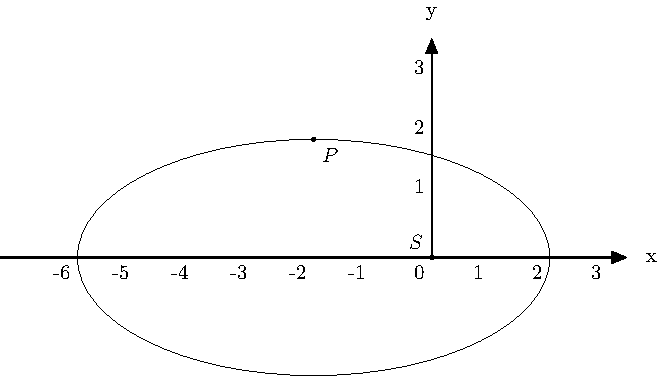
\includegraphics{images/2body}}
\resizebox{0.3\textwidth}{!}{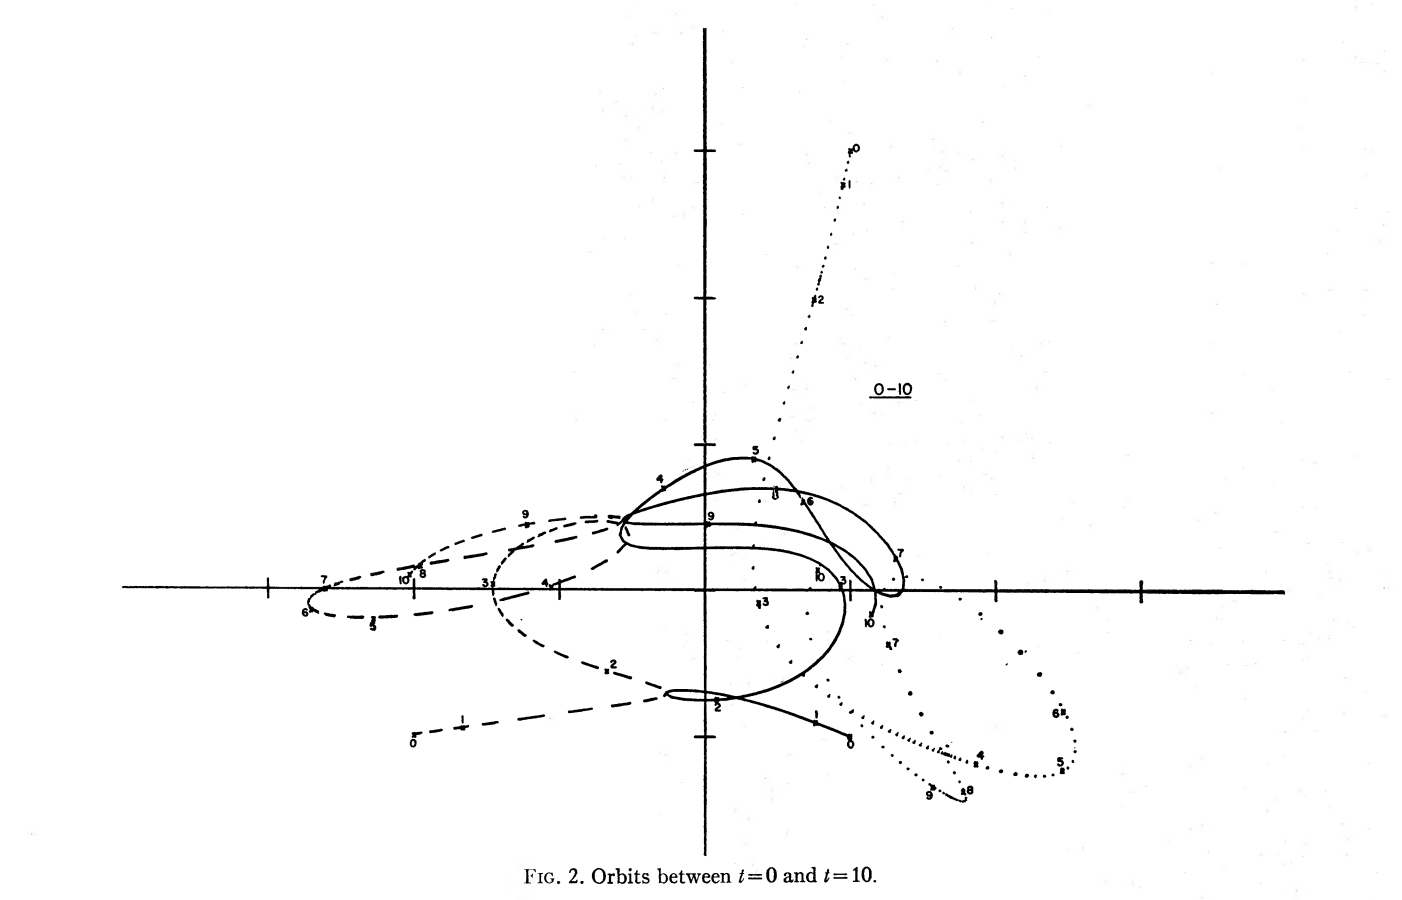
\includegraphics{images/3body}}
\resizebox{0.3\textwidth}{!}{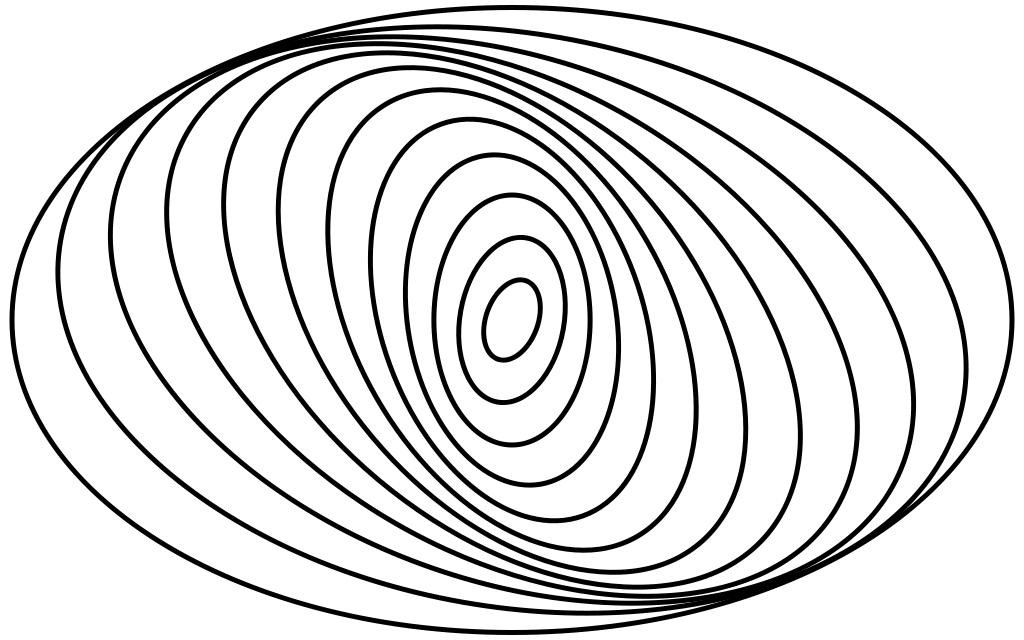
\includegraphics{images/spiral_galaxy_arms_diagram}}
\caption{a 2-body orbit; a 3-body orbit; dense wave of spiral galaxies}
\end{figure}
\end{frame}

\begin{frame}
\frametitle{Overparameterization}
\end{frame}

\begin{frame}
\frametitle{Expressiveness of dimensions}

\end{frame}

\begin{frame}
\frametitle{A neglected possibility}
\end{frame}

\begin{frame}
\frametitle{Random walks}
\end{frame}

\begin{frame}
\frametitle{Relation and parallelism}
\end{frame}

\begin{frame}
\frametitle{But how?}
\end{frame}

\begin{frame}
\maketitle
\end{frame}

\begin{frame}
\frametitle{Table of Contents}
\tableofcontents
\end{frame}

\section{The first glimpse}

\begin{frame}
\frametitle{The first glimpse}
\begin{figure}[ht]\centering
\resizebox{0.5\textwidth}{!}{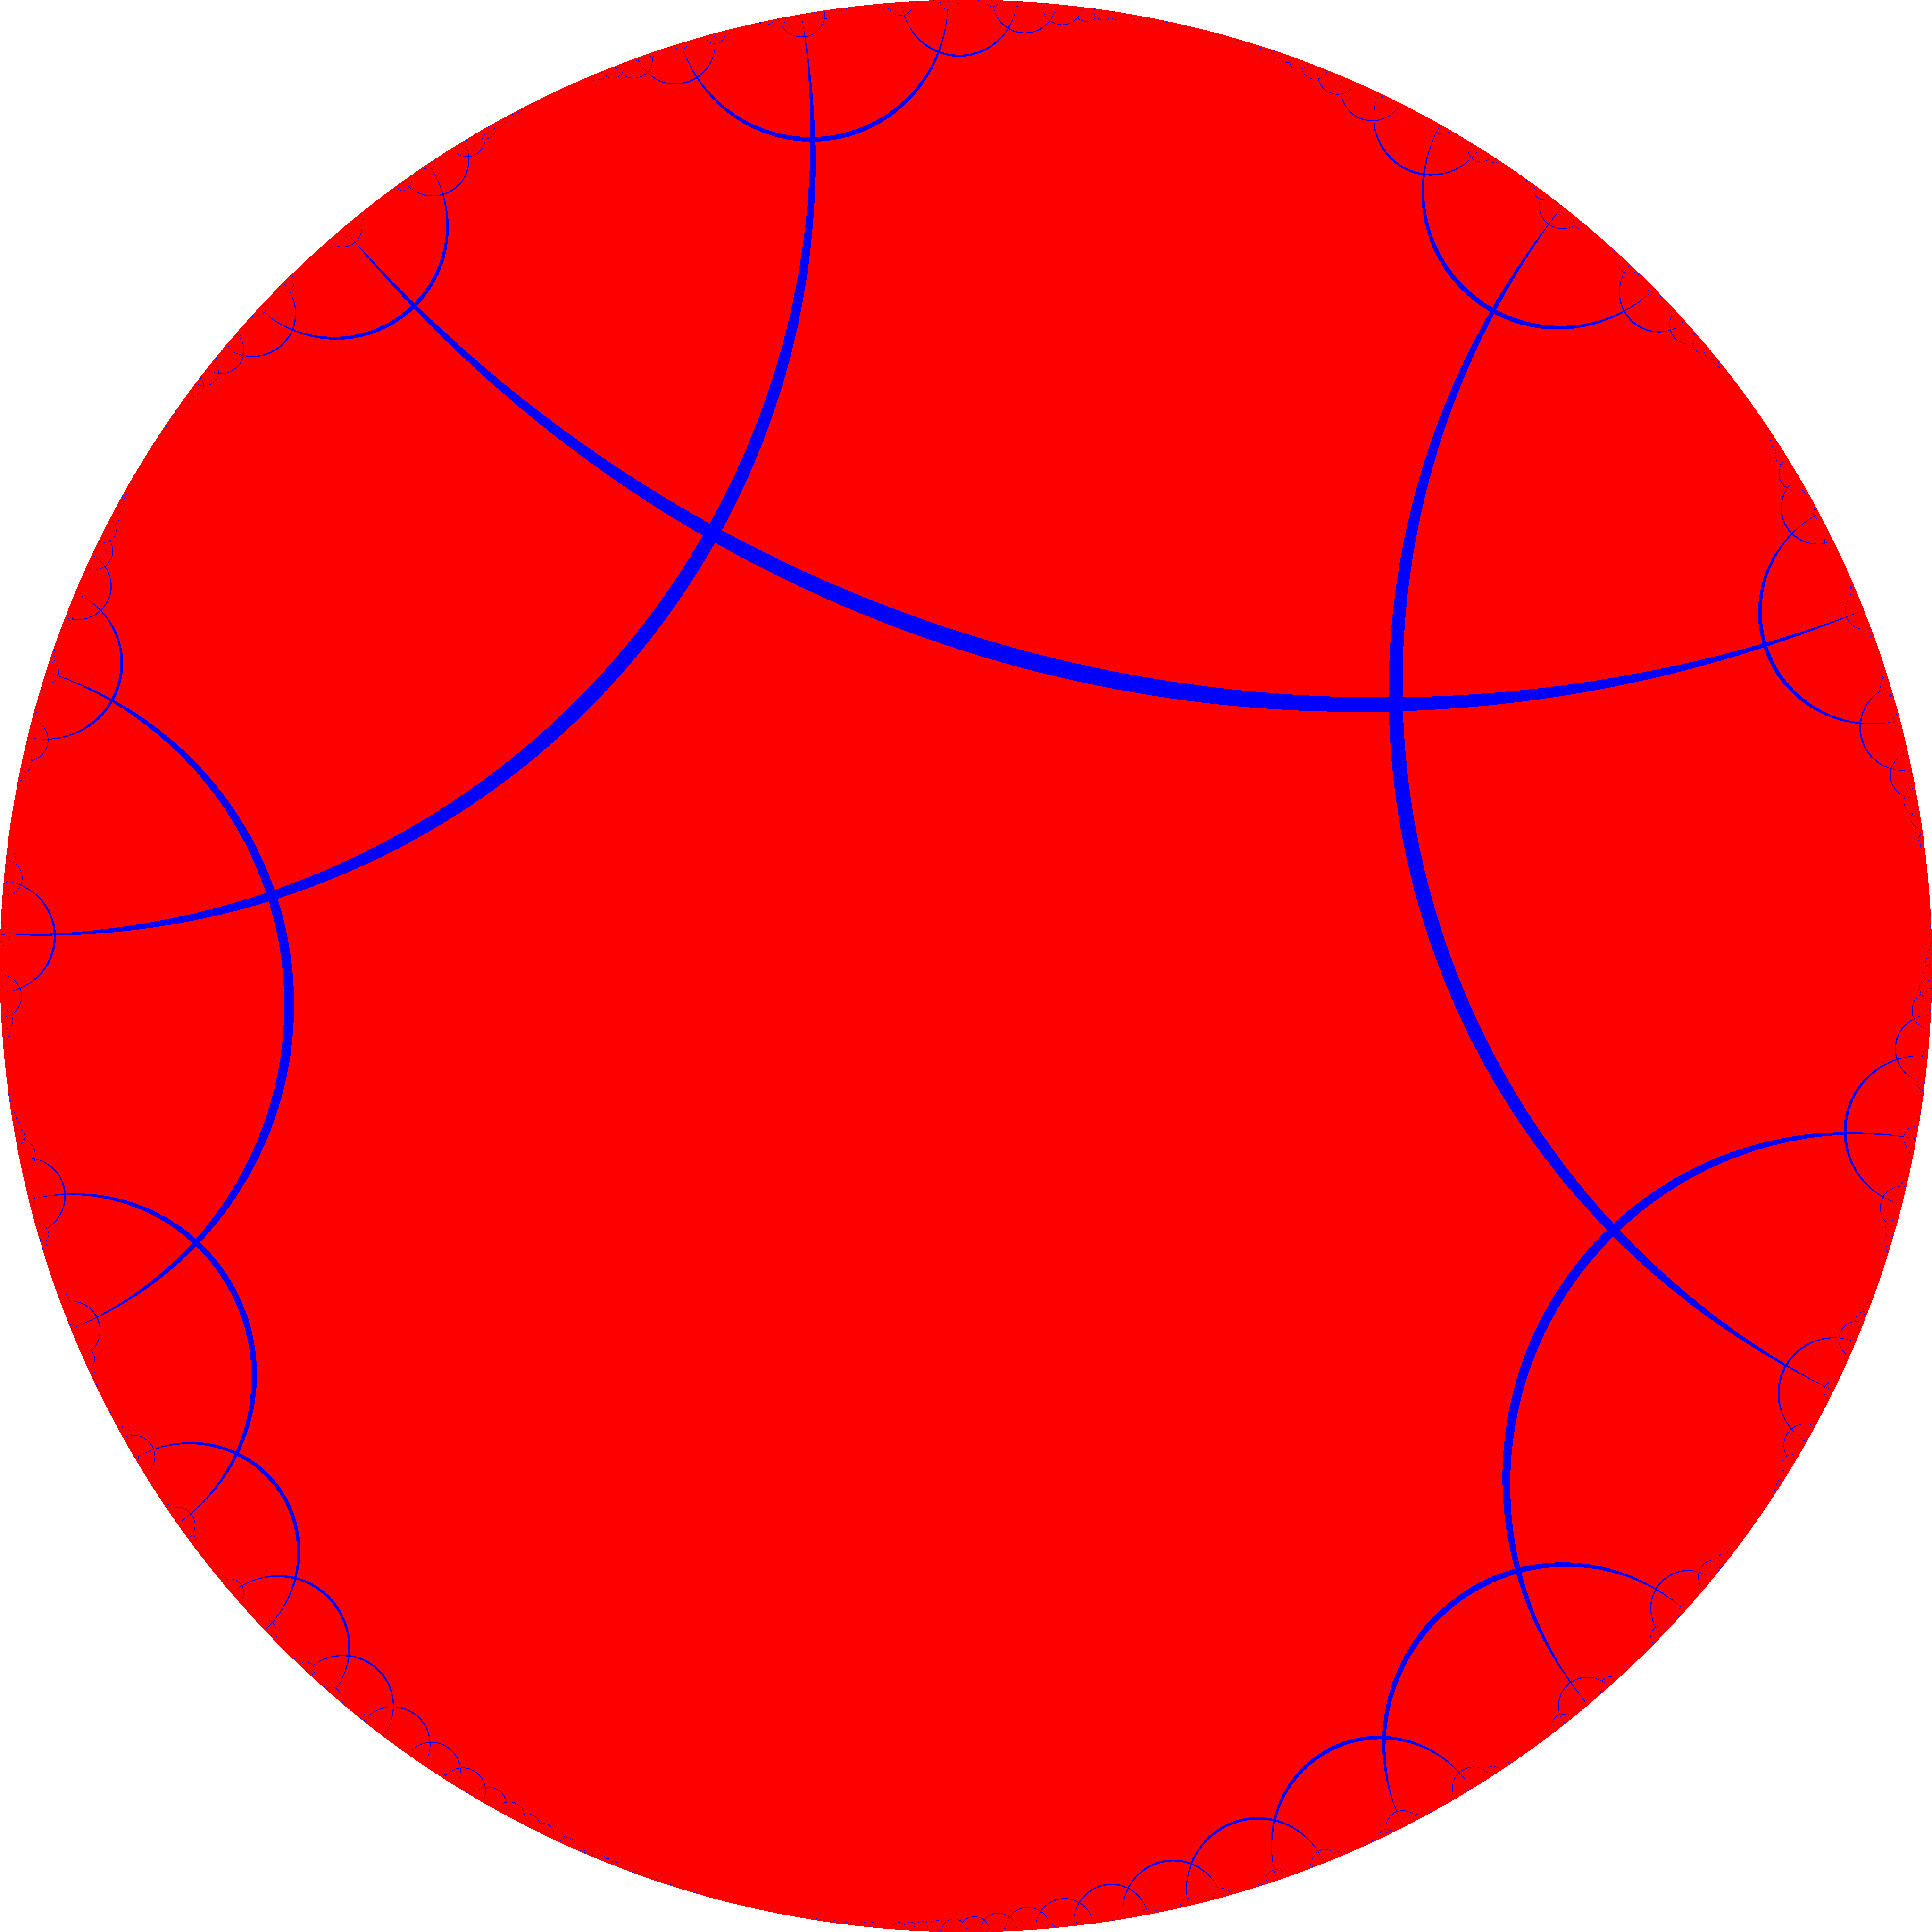
\includegraphics{images/t4096}}
\end{figure}
\end{frame}

\begin{frame}
\frametitle{The beginning point}
The famous example of word2vec
\begin{figure}[ht]
\centering
\resizebox{0.5\textwidth}{!}{
\begin{tikzpicture}[x=0.5cm,y=0.5cm,z=0.3cm,>=stealth]
\draw[->] (xyz cs:x=-7.0) -- (xyz cs:x=7.0) node[above] {$x_0$};
\draw[->] (xyz cs:y=0) -- (xyz cs:y=7.0) node[right] {$x_n$};
\draw[->] (xyz cs:z=-7.0) -- (xyz cs:z=7.0) node[above] {$x_i$};

\node[fill,circle,inner sep=1.5pt,label={left:$king$}] (p) at (xyz cs:x=-3.0, y=3.0, z=-3.0) {};
\node[fill,circle,inner sep=1.5pt,label={right:$man$}] (q) at (xyz cs:x=2.0, y=-3.0, z=3.0) {};
\node[fill,circle,inner sep=1.5pt,label={left:$queen$}] (r) at (xyz cs:x=-3.0, y=3.0, z=3.0) {};
\node[fill,circle,inner sep=1.5pt,label={right:$woman$}] (s) at (xyz cs:x=2.0, y=-3.0, z=9.0) {};
\draw[dashed, blue] (p) -- (q);
\draw[dashed, blue] (r) -- (s);
\draw[dashed, red] (p) -- (r);
\draw[dashed, red] (q) -- (s);
\end{tikzpicture}
}
\caption{regulairty of word2vec}
\label{fig:regulairty-of-word2vec}
\end{figure}
\end{frame}

\begin{frame}
\frametitle{The case of numbers}
\[
(\alpha + 1) \times 2 \neq \alpha \times 2 + 1
\]

\begin{figure}[ht]
\centering
\resizebox{0.5\textwidth}{!}{
\begin{tikzpicture}[x=0.5cm,y=0.5cm,z=0.3cm,>=stealth]
\draw[->] (xyz cs:x=-7.0) -- (xyz cs:x=7.0) node[above] {$x_0$};
\draw[->] (xyz cs:y=0) -- (xyz cs:y=7.0) node[right] {$x_n$};
\draw[->] (xyz cs:z=-7.0) -- (xyz cs:z=7.0) node[above] {$x_i$};

\node[fill,circle,inner sep=1.5pt,label={left:$\alpha$}] (p) at (xyz cs:x=-3.0, y=3.0, z=-3.0) {};
\node[fill,circle,inner sep=1.5pt,label={right:$\alpha+1$}] (q) at (xyz cs:x=2.0, y=-3.0, z=3.0) {};
\node[fill,circle,inner sep=1.5pt,label={left:$\alpha \times 2$}] (r) at (xyz cs:x=-3.0, y=3.0, z=3.0) {};
\node[fill,circle,inner sep=1.5pt,label={right:$(\alpha + 1) \times 2 \neq \alpha \times 2 + 1$}] (s) at (xyz cs:x=2.0, y=-3.0, z=9.0) {};
\draw[dashed, blue] (p) -- (q);
\draw[dashed, blue] (r) -- (s);
\draw[dashed, red] (p) -- (r);
\draw[dashed, red] (q) -- (s);
\end{tikzpicture}
}
\caption{contradiction of numbers in Euclidean space}
\label{fig:contradiction-of-numbers}
\end{figure}

\end{frame}

\begin{frame}
\frametitle{One arrangement in hyperbolic space}
\begin{figure}[ht]\centering
\resizebox{0.5\textwidth}{!}{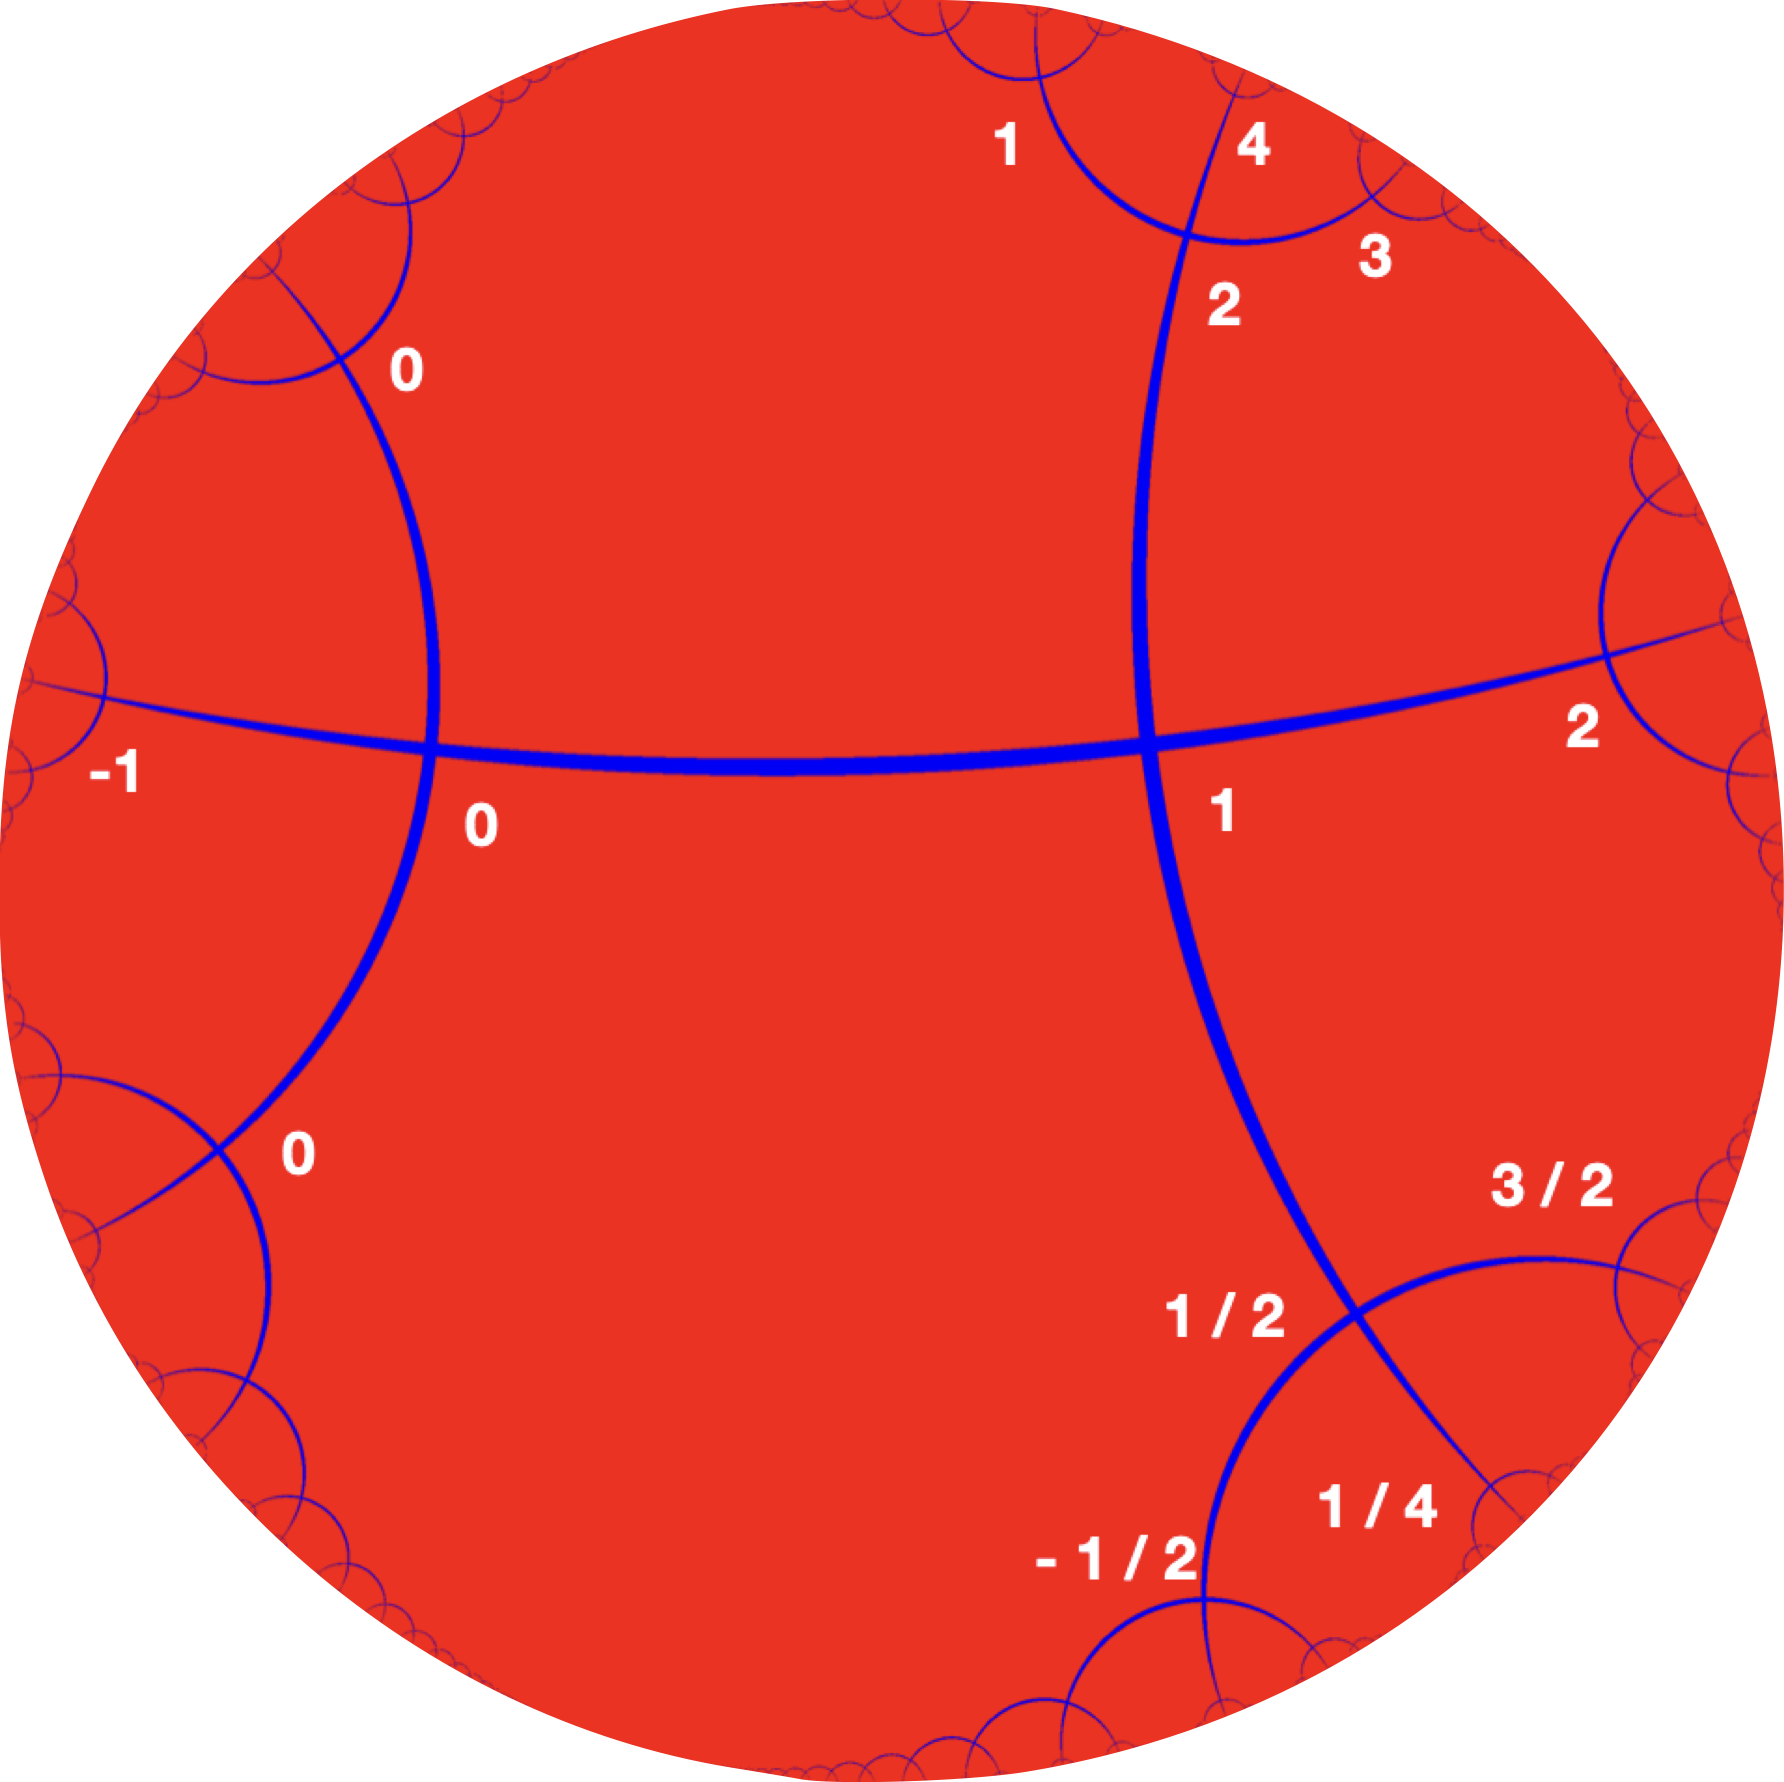
\includegraphics{images/assignment2}}
\end{figure}
\end{frame}

\begin{frame}
\frametitle{Another arrangement in hyperbolic space}

\[
    a = - \frac{x}{y}
\]

\begin{figure}[ht]
\centering
\resizebox{0.7\textwidth}{!}{
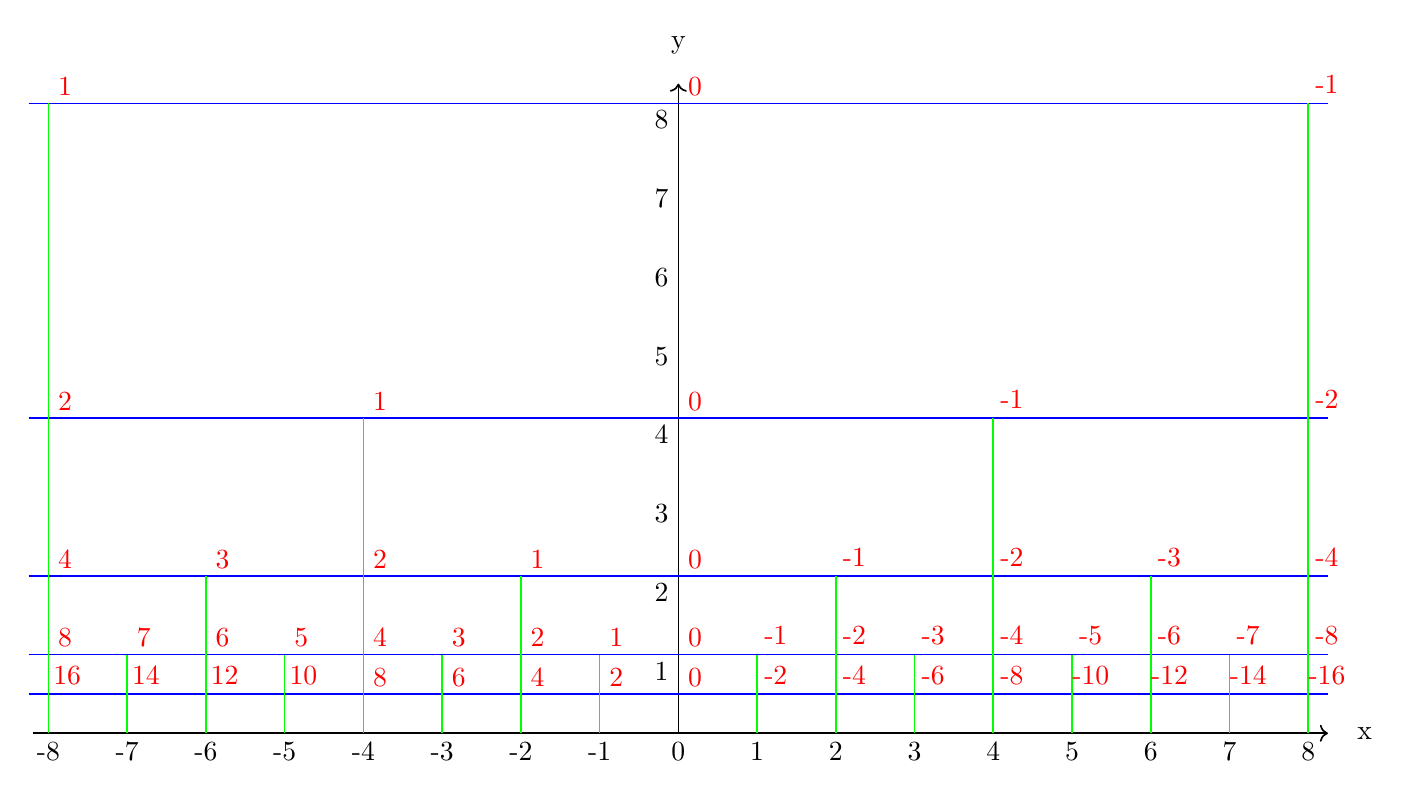
\begin{tikzpicture}
\draw [black, line width=0.6pt, ->] (0,0) to[out=90,in=270] (0,8.25);
\node [anchor=south] at (0,8.5) {y};
\draw [black, line width=0.6pt, ->] (-8.2,0) to[out=0,in=180] (8.25,0);
\node [anchor=west] at (8.5,0) {x};
\foreach \x in {-8,-7,-6,-5,-4,-3,-2,-1,0,1,2,3,4,5,6,7,8}
  \node [anchor=north] at (\x,0) {\x};
\foreach \y in {1,2,3,4,5,6,7,8}
  \node [anchor=45] at (0,\y) {\y};

\draw [blue, line width=0.6pt] (-8.25,0.5) to[out=0,in=180] (8.25,0.5);
\draw [blue, line width=0.6pt] (-8.25,1) to[out=0,in=180] (8.25,1);
\draw [blue, line width=0.6pt] (-8.25,2) to[out=0,in=180] (8.25,2);
\draw [blue, line width=0.6pt] (-8.25,4) to[out=0,in=180] (8.25,4);
\draw [blue, line width=0.6pt] (-8.25,8) to[out=0,in=180] (8.25,8);

\draw [green, line width=0.6pt] (-8,0) to[out=90,in=270] (-8,1);
\draw [green, line width=0.6pt] (-7,0) to[out=90,in=270] (-7,1);
\draw [green, line width=0.6pt] (-6,0) to[out=90,in=270] (-6,1);
\draw [green, line width=0.6pt] (-5,0) to[out=90,in=270] (-5,1);
\draw [green, line width=0.6pt] (-4,0) to[out=90,in=270] (-4,1);
\draw [green, line width=0.6pt] (-3,0) to[out=90,in=270] (-3,1);
\draw [green, line width=0.6pt] (-2,0) to[out=90,in=270] (-2,1);
\draw [green, line width=0.6pt] (-1,0) to[out=90,in=270] (-1,1);
\draw [green, line width=0.6pt] (1,0) to[out=90,in=270] (1,1);
\draw [green, line width=0.6pt] (2,0) to[out=90,in=270] (2,1);
\draw [green, line width=0.6pt] (3,0) to[out=90,in=270] (3,1);
\draw [green, line width=0.6pt] (4,0) to[out=90,in=270] (4,1);
\draw [green, line width=0.6pt] (5,0) to[out=90,in=270] (5,1);
\draw [green, line width=0.6pt] (6,0) to[out=90,in=270] (6,1);
\draw [green, line width=0.6pt] (7,0) to[out=90,in=270] (7,1);
\draw [green, line width=0.6pt] (8,0) to[out=90,in=270] (8,1);

\draw [green, line width=0.6pt] (-8,1) to[out=90,in=270] (-8,2);
\draw [green, line width=0.6pt] (-6,1) to[out=90,in=270] (-6,2);
\draw [green, line width=0.6pt] (-4,1) to[out=90,in=270] (-4,2);
\draw [green, line width=0.6pt] (-2,1) to[out=90,in=270] (-2,2);
\draw [green, line width=0.6pt] (2,1) to[out=90,in=270] (2,2);
\draw [green, line width=0.6pt] (4,1) to[out=90,in=270] (4,2);
\draw [green, line width=0.6pt] (6,1) to[out=90,in=270] (6,2);
\draw [green, line width=0.6pt] (8,1) to[out=90,in=270] (8,2);

\draw [green, line width=0.6pt] (-8,2) to[out=90,in=270] (-8,4);
\draw [green, line width=0.6pt] (-4,2) to[out=90,in=270] (-4,4);
\draw [green, line width=0.6pt] (4,2) to[out=90,in=270] (4,4);
\draw [green, line width=0.6pt] (8,2) to[out=90,in=270] (8,4);

\draw [green, line width=0.6pt] (-8,4) to[out=90,in=270] (-8,8);
\draw [green, line width=0.6pt] (8,4) to[out=90,in=270] (8,8);

\node [anchor=225, red] at (-8,0.5) {16};
\node [anchor=225, red] at (-7,0.5) {14};
\node [anchor=225, red] at (-6,0.5) {12};
\node [anchor=225, red] at (-5,0.5) {10};
\node [anchor=225, red] at (-4,0.5) {8};
\node [anchor=225, red] at (-3,0.5) {6};
\node [anchor=225, red] at (-2,0.5) {4};
\node [anchor=225, red] at (-1,0.5) {2};
\node [anchor=225, red] at (0,0.5) {0};
\node [anchor=225, red] at (1,0.5) {-2};
\node [anchor=225, red] at (2,0.5) {-4};
\node [anchor=225, red] at (3,0.5) {-6};
\node [anchor=225, red] at (4,0.5) {-8};
\node [anchor=225, red] at (5,0.5) {-10};
\node [anchor=225, red] at (6,0.5) {-12};
\node [anchor=225, red] at (7,0.5) {-14};
\node [anchor=225, red] at (8,0.5) {-16};

\node [anchor=225, red] at (-8,1) {8};
\node [anchor=225, red] at (-7,1) {7};
\node [anchor=225, red] at (-6,1) {6};
\node [anchor=225, red] at (-5,1) {5};
\node [anchor=225, red] at (-4,1) {4};
\node [anchor=225, red] at (-3,1) {3};
\node [anchor=225, red] at (-2,1) {2};
\node [anchor=225, red] at (-1,1) {1};
\node [anchor=225, red] at (0,1) {0};
\node [anchor=225, red] at (1,1) {-1};
\node [anchor=225, red] at (2,1) {-2};
\node [anchor=225, red] at (3,1) {-3};
\node [anchor=225, red] at (4,1) {-4};
\node [anchor=225, red] at (5,1) {-5};
\node [anchor=225, red] at (6,1) {-6};
\node [anchor=225, red] at (7,1) {-7};
\node [anchor=225, red] at (8,1) {-8};

\node [anchor=225, red] at (-8,2) {4};
\node [anchor=225, red] at (-6,2) {3};
\node [anchor=225, red] at (-4,2) {2};
\node [anchor=225, red] at (-2,2) {1};
\node [anchor=225, red] at (0,2) {0};
\node [anchor=225, red] at (2,2) {-1};
\node [anchor=225, red] at (4,2) {-2};
\node [anchor=225, red] at (6,2) {-3};
\node [anchor=225, red] at (8,2) {-4};

\node [anchor=225, red] at (-8,4) {2};
\node [anchor=225, red] at (-4,4) {1};
\node [anchor=225, red] at (0,4) {0};
\node [anchor=225, red] at (4,4) {-1};
\node [anchor=225, red] at (8,4) {-2};

\node [anchor=225, red] at (-8,8) {1};
\node [anchor=225, red] at (0,8) {0};
\node [anchor=225, red] at (8,8) {-1};

\end{tikzpicture}
}
\label{fig:gridex0}
\end{figure}
\end{frame}

\begin{frame}
\frametitle{Encoding threadlike expressions as paths}

\begin{itemize}
    \item black line $1 \times 8 - 5 = 3$
\end{itemize}

\begin{figure}[ht]
\centering
\resizebox{0.7\textwidth}{!}{
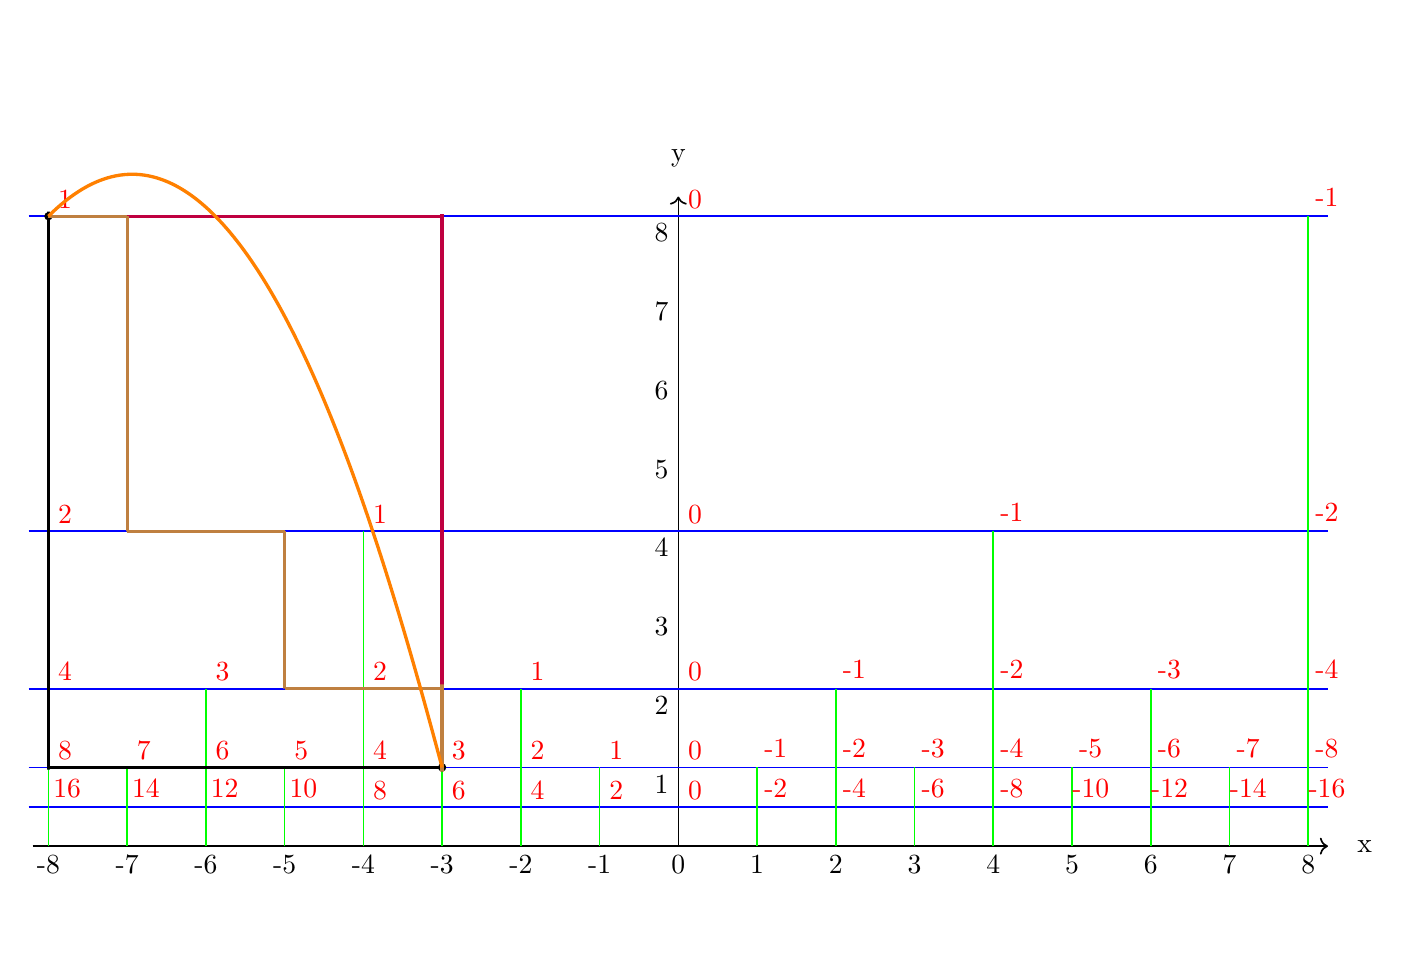
\begin{tikzpicture}
\draw [black, line width=0.6pt, ->] (0,0) to[out=90,in=270] (0,8.25);
\node [anchor=south] at (0,8.5) {y};
\draw [black, line width=0.6pt, ->] (-8.2,0) to[out=0,in=180] (8.25,0);
\node [anchor=west] at (8.5,0) {x};
\foreach \x in {-8,-7,-6,-5,-4,-3,-2,-1,0,1,2,3,4,5,6,7,8}
  \node [anchor=north] at (\x,0) {\x};
\foreach \y in {1,2,3,4,5,6,7,8}
  \node [anchor=45] at (0,\y) {\y};

\draw [blue, line width=0.6pt] (-8.25,0.5) to[out=0,in=180] (8.25,0.5);
\draw [blue, line width=0.6pt] (-8.25,1) to[out=0,in=180] (8.25,1);
\draw [blue, line width=0.6pt] (-8.25,2) to[out=0,in=180] (8.25,2);
\draw [blue, line width=0.6pt] (-8.25,4) to[out=0,in=180] (8.25,4);
\draw [blue, line width=0.6pt] (-8.25,8) to[out=0,in=180] (8.25,8);

\draw [green, line width=0.6pt] (-8,0) to[out=90,in=270] (-8,1);
\draw [green, line width=0.6pt] (-7,0) to[out=90,in=270] (-7,1);
\draw [green, line width=0.6pt] (-6,0) to[out=90,in=270] (-6,1);
\draw [green, line width=0.6pt] (-5,0) to[out=90,in=270] (-5,1);
\draw [green, line width=0.6pt] (-4,0) to[out=90,in=270] (-4,1);
\draw [green, line width=0.6pt] (-3,0) to[out=90,in=270] (-3,1);
\draw [green, line width=0.6pt] (-2,0) to[out=90,in=270] (-2,1);
\draw [green, line width=0.6pt] (-1,0) to[out=90,in=270] (-1,1);
\draw [green, line width=0.6pt] (1,0) to[out=90,in=270] (1,1);
\draw [green, line width=0.6pt] (2,0) to[out=90,in=270] (2,1);
\draw [green, line width=0.6pt] (3,0) to[out=90,in=270] (3,1);
\draw [green, line width=0.6pt] (4,0) to[out=90,in=270] (4,1);
\draw [green, line width=0.6pt] (5,0) to[out=90,in=270] (5,1);
\draw [green, line width=0.6pt] (6,0) to[out=90,in=270] (6,1);
\draw [green, line width=0.6pt] (7,0) to[out=90,in=270] (7,1);
\draw [green, line width=0.6pt] (8,0) to[out=90,in=270] (8,1);

\draw [green, line width=0.6pt] (-8,1) to[out=90,in=270] (-8,2);
\draw [green, line width=0.6pt] (-6,1) to[out=90,in=270] (-6,2);
\draw [green, line width=0.6pt] (-4,1) to[out=90,in=270] (-4,2);
\draw [green, line width=0.6pt] (-2,1) to[out=90,in=270] (-2,2);
\draw [green, line width=0.6pt] (2,1) to[out=90,in=270] (2,2);
\draw [green, line width=0.6pt] (4,1) to[out=90,in=270] (4,2);
\draw [green, line width=0.6pt] (6,1) to[out=90,in=270] (6,2);
\draw [green, line width=0.6pt] (8,1) to[out=90,in=270] (8,2);

\draw [green, line width=0.6pt] (-8,2) to[out=90,in=270] (-8,4);
\draw [green, line width=0.6pt] (-4,2) to[out=90,in=270] (-4,4);
\draw [green, line width=0.6pt] (4,2) to[out=90,in=270] (4,4);
\draw [green, line width=0.6pt] (8,2) to[out=90,in=270] (8,4);

\draw [green, line width=0.6pt] (-8,4) to[out=90,in=270] (-8,8);
\draw [green, line width=0.6pt] (8,4) to[out=90,in=270] (8,8);

\node [anchor=225, red] at (-8,0.5) {16};
\node [anchor=225, red] at (-7,0.5) {14};
\node [anchor=225, red] at (-6,0.5) {12};
\node [anchor=225, red] at (-5,0.5) {10};
\node [anchor=225, red] at (-4,0.5) {8};
\node [anchor=225, red] at (-3,0.5) {6};
\node [anchor=225, red] at (-2,0.5) {4};
\node [anchor=225, red] at (-1,0.5) {2};
\node [anchor=225, red] at (0,0.5) {0};
\node [anchor=225, red] at (1,0.5) {-2};
\node [anchor=225, red] at (2,0.5) {-4};
\node [anchor=225, red] at (3,0.5) {-6};
\node [anchor=225, red] at (4,0.5) {-8};
\node [anchor=225, red] at (5,0.5) {-10};
\node [anchor=225, red] at (6,0.5) {-12};
\node [anchor=225, red] at (7,0.5) {-14};
\node [anchor=225, red] at (8,0.5) {-16};

\node [anchor=225, red] at (-8,1) {8};
\node [anchor=225, red] at (-7,1) {7};
\node [anchor=225, red] at (-6,1) {6};
\node [anchor=225, red] at (-5,1) {5};
\node [anchor=225, red] at (-4,1) {4};
\node [anchor=225, red] at (-3,1) {3};
\node [anchor=225, red] at (-2,1) {2};
\node [anchor=225, red] at (-1,1) {1};
\node [anchor=225, red] at (0,1) {0};
\node [anchor=225, red] at (1,1) {-1};
\node [anchor=225, red] at (2,1) {-2};
\node [anchor=225, red] at (3,1) {-3};
\node [anchor=225, red] at (4,1) {-4};
\node [anchor=225, red] at (5,1) {-5};
\node [anchor=225, red] at (6,1) {-6};
\node [anchor=225, red] at (7,1) {-7};
\node [anchor=225, red] at (8,1) {-8};

\node [anchor=225, red] at (-8,2) {4};
\node [anchor=225, red] at (-6,2) {3};
\node [anchor=225, red] at (-4,2) {2};
\node [anchor=225, red] at (-2,2) {1};
\node [anchor=225, red] at (0,2) {0};
\node [anchor=225, red] at (2,2) {-1};
\node [anchor=225, red] at (4,2) {-2};
\node [anchor=225, red] at (6,2) {-3};
\node [anchor=225, red] at (8,2) {-4};

\node [anchor=225, red] at (-8,4) {2};
\node [anchor=225, red] at (-4,4) {1};
\node [anchor=225, red] at (0,4) {0};
\node [anchor=225, red] at (4,4) {-1};
\node [anchor=225, red] at (8,4) {-2};

\node [anchor=225, red] at (-8,8) {1};
\node [anchor=225, red] at (0,8) {0};
\node [anchor=225, red] at (8,8) {-1};

\node[circle,fill=black,inner sep=1pt,minimum size=3pt] (a) at (-8,8) {};
\node[circle,fill=black,inner sep=1pt,minimum size=3pt] (b) at (-3,1) {};

\draw [black, line width=1.2pt] (-8,7.7) to[out=90,in=270] (-8,1.33);
\draw [black, line width=1.2pt] (-8,1) to[out=0,in=180] (-3,1);

\draw [purple, line width=1.2pt] (-8,8) to[out=0,in=180] (-3,8);
\draw [purple, line width=1.2pt] (-3,7.67) to[out=90,in=270] (-3,1.33);

\draw [brown, line width=1.2pt] (-8,8) to[out=0,in=180] (-7,8);
\draw [brown, line width=1.2pt] (-7,7.8) to[out=90,in=270] (-7,4.2);
\draw [brown, line width=1.2pt] (-7,4) to[out=0,in=180] (-5,4);
\draw [brown, line width=1.2pt] (-5,3.9) to[out=90,in=270] (-5,2.1);
\draw [brown, line width=1.2pt] (-5,2) to[out=0,in=180] (-3,2);
\draw [brown, line width=1.2pt] (-3,2) to[out=90,in=270] (-3,1);

\draw [orange, line width=1.2pt] (-8,8) to[out=45,in=105] (-3,1);

\end{tikzpicture}
}
\label{fig:pathex1}
\end{figure}

\end{frame}

\begin{frame}
\frametitle{The flow equation}

Suppose we have a base point $a_0$, and we step a small distance away from $a_0$.

Addition first

\[
    a_{\delta} = (a_0 + \mu \epsilon \cos \theta)e^{\lambda \epsilon \sin \theta}
\]

Multiplication first

\[
    a_{\delta} = a_0 e^{\lambda \epsilon \sin \theta} + \mu \epsilon \cos \theta
\]

\end{frame}

\begin{frame}
\frametitle{The flow equation}

Both formula can be simplified to the same result:

\[
    a_{\delta} = a_0 + \epsilon (a_0 \lambda \sin \theta + \mu \cos \theta)
\]

Then, we have the following equation:

\[
    \frac{1}{\delta} (a_{\delta} - a_0) = \frac{\epsilon}{\delta} (\mu \cos \theta + a_0 \lambda \sin \theta)
\]

When both $\delta$ and $\epsilon$ are towards zero, we get $da / dt$, and hence

\[
    \frac{da}{dt} = u (\mu \cos \theta + a \lambda \sin \theta)
\]

Or, we can change it to another form

\begin{equation}
    \frac{da}{ds} = \mu \cos \theta + a \lambda \sin \theta\label{eq:flow}
\end{equation}

\end{frame}


\section{Fundamental problems}

\begin{frame}
\frametitle{Fundamental problems}
\begin{figure}[ht]\centering
\resizebox{0.7\textwidth}{!}{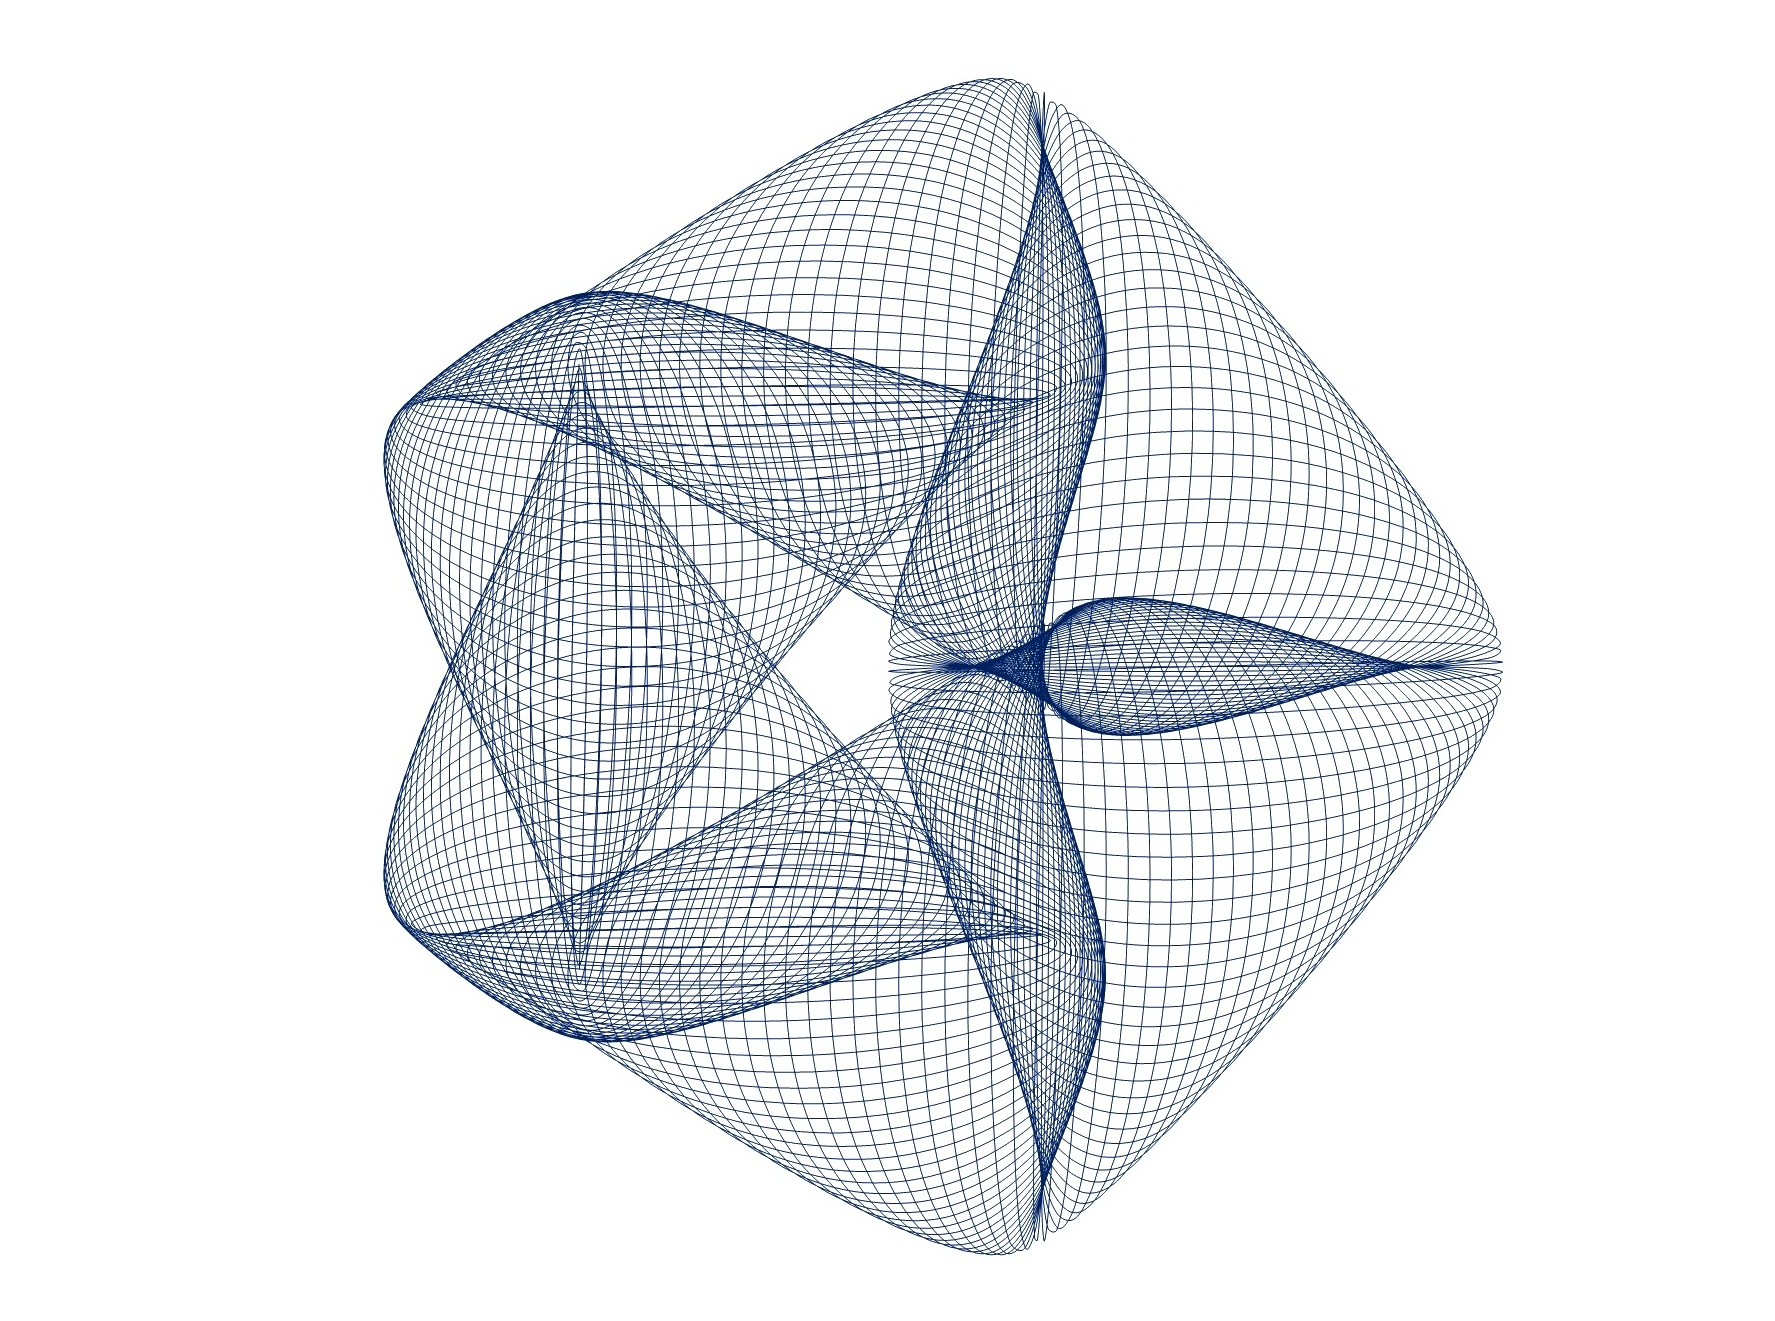
\includegraphics{images/param_curve}}
\end{figure}
\end{frame}

\begin{frame}
\frametitle{What is an arithmetic expression?}

Giving an arithmetic expression, we can parse it into a syntax tree. For example, the expression

\begin{equation}
(((((1 \times 2) \times 2) - 1) \times (2 + 1)) - 6)\label{eq:equation}
\end{equation}

and the parsed syntax tree

\begin{figure}[ht]
\centering
\resizebox{0.4\textheight}{!}{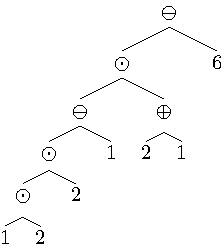
\includegraphics{images/02-example-expression-syntax-tree.pdf}}
\caption{a tree representation of an arithmetic expression}\label{fig:syntaxtree}\label{fig:figure}
\end{figure}
\end{frame}

\begin{frame}
\frametitle{A definition of arithmetic expression}
\begin{definition}\label{def:arithmetic-expression}
    An arithmetic expression $a$ over $\mathbb{Q}$ is a structure given by the following production rules:
\begin{equation}\label{eq:productionrule}
\begin{aligned}
a &\longleftarrow x\\
a &\longleftarrow ( a + a )\\
a &\longleftarrow ( a - a )\\
a &\longleftarrow ( a \times a )\\
a &\longleftarrow ( a \div a )
\end{aligned}
\end{equation}
    where $x \in \mathbb{Q}$, and we denote this as $a \in \mathbb{E} \left [\mathbb{Q} \right ]$.
\end{definition}
\end{frame}

\begin{frame}
\frametitle{Evaluation of arithmetic expression}
We can define evaluation $\nu(a)$ of $a$ recursively as follows:
\begin{itemize}
  \item Constant leaf: for any $x \in \mathbb{Q}$, $\nu(x) = x$.
  \item Compositional node by $+$: For any $(a + b)$, $\nu((a + b)) = \nu(a) + \nu(b)$.
  \item Compositional node by $-$: For any $(a - b)$, $\nu((a - b)) = \nu(a) - \nu(b)$.
  \item Compositional node by $\times$: For any $(a \times b)$, $\nu((a \times b)) = \nu(a) \nu(b)$.
  \item Compositional node by $\div$: For any $(a \div b)$, if $\nu(b) \neq 0$, then $\nu((a \div b)) = \nu(a) / \nu(b)$.
\end{itemize}
\end{frame}

\begin{frame}
\frametitle{Syntactic vs. Semantic}
A careful reader may have noticed that the definition~\ref{def:arithmetic-expression} is based on rational numbers $\mathbb{Q}$.
Why can't we use real numbers $\mathbb{R}$ instead?
The answer is that syntactically valid expressions may not be semantically valid.
Dividing by zero can lead to invalid expressions, and the evaluation of the expression cannot be defined in this situation.
Therefore, in real numbers, an expression may be syntactically valid but semantically not valid,
and there is no algorithm that can decide whether an expression is semantically valid or not.
\end{frame}

\begin{frame}
\frametitle{Topological arithmetic expression space}
\begin{enumerate}
    \item Convergence geometrically can lead to convergence of arithmetic evaluation
    \item The arithmetic evaluation can be extended to the whole topological space continuously
\end{enumerate}

\end{frame}

\begin{frame}
\frametitle{Topological arithmetic expression space}
We denote the set of all well-defined arithmetic expressions over the field of rational numbers $\mathbb{Q}$ as $\mathbb{A}$, where $\nu$ is a function from $\mathbb{A}$ to $\mathbb{Q}$.
\begin{definition}
There is a countable dense set $G$ on the topological space $\mathcal{A}$, and there exists an injection $\kappa: G \to \mathbb{A}$ between this dense set and the well-defined arithmetic expressions.
We denote the image of this mapping as $\kappa(G) = \mathbb{K}$. If for any point $x \in \mathcal{A}$,
and any two sequences of points $y_i \in G$ and $w_j \in G$, when $y_i$ converges to $x$ and $w_j$ also converges to $x$,
the sequences of points over the rational numbers $\nu(\kappa(y_i))$ and $\nu(\kappa(w_j))$ both converge to the same real number; in this case, we can naturally make an extension:
\begin{itemize}
\item Extend $G$ to a closed set $\bar{G}$ on $\mathcal{A}$;
\item Extend $\nu$ to a mapping $\bar{\nu}$ from $\bar{\mathbb{K}}$ to the real numbers $\mathbb{R}$;
\end{itemize}
If this extended valuation function $\bar{\nu}$ is a continuous function, then we call the topological space $\mathcal{A}$ a topological arithmetic expression space. $G$ is referred to as the grid on $\mathcal{A}$.
\end{definition}

\end{frame}

\begin{frame}
\frametitle{Classification problem}
\emph{Local structure}: decided by the flow equation~\ref{eq:flow}.

\emph{Classification of the global structure}

\end{frame}

\begin{frame}
\frametitle{Eigenfunction of Laplacian}
On the hyperbolic plane
\[
ds^2 = \frac{dx^2 + dy^2}{y^2}
\]

the Laplacian is
\[
\Delta = - y^2 (\frac{\partial^2}{\partial x^2} + \frac{\partial^2}{\partial y^2})
\]

Given

\begin{equation}
A = - \frac{x}{y}
\end{equation}

We have

$$
\Delta A = - y^2 (\frac{\partial^2}{\partial x^2} A + \frac{\partial^2}{\partial y^2} A) = y^2 (\frac{1}{\partial y} (\frac{1}{\partial y} \frac{x}{y})) = 2 A
$$

\end{frame}

\section{Further topics}

\begin{frame}
\frametitle{Further topics}
\begin{figure}[ht]\centering
\resizebox{0.5\textwidth}{!}{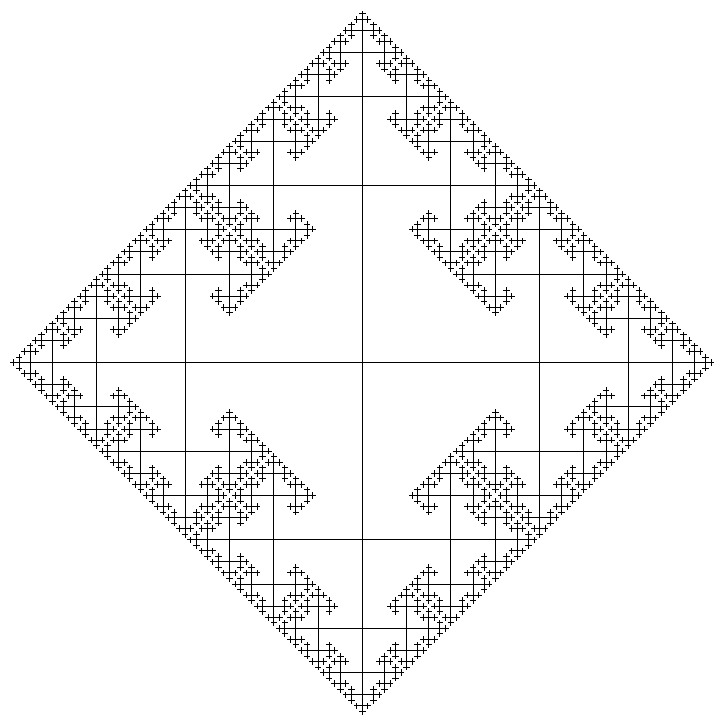
\includegraphics{images/cayley4}}
\end{figure}
\end{frame}

\begin{frame}
\frametitle{A jigsaw by Riemann mapping?}
\begin{figure}[ht]\centering
\resizebox{0.7\textwidth}{!}{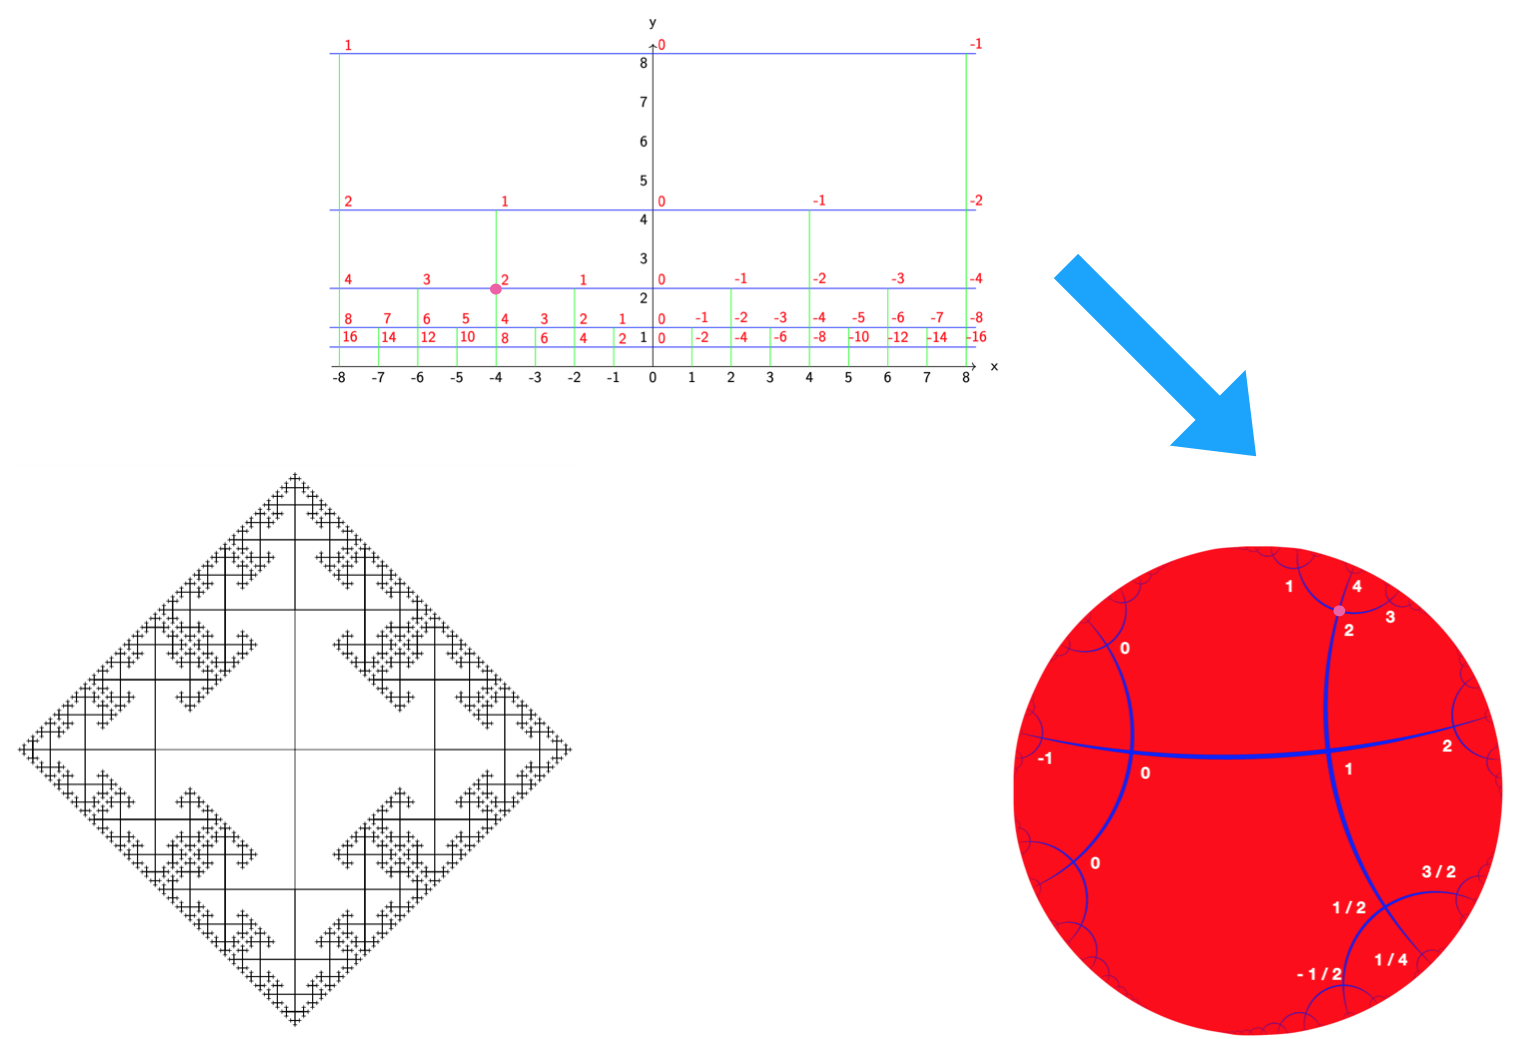
\includegraphics{images/jigsaw-riemann}}
\end{figure}
\end{frame}

\begin{frame}
\frametitle{Tube structure?}
\begin{figure}[ht]\centering
\resizebox{0.8\textwidth}{!}{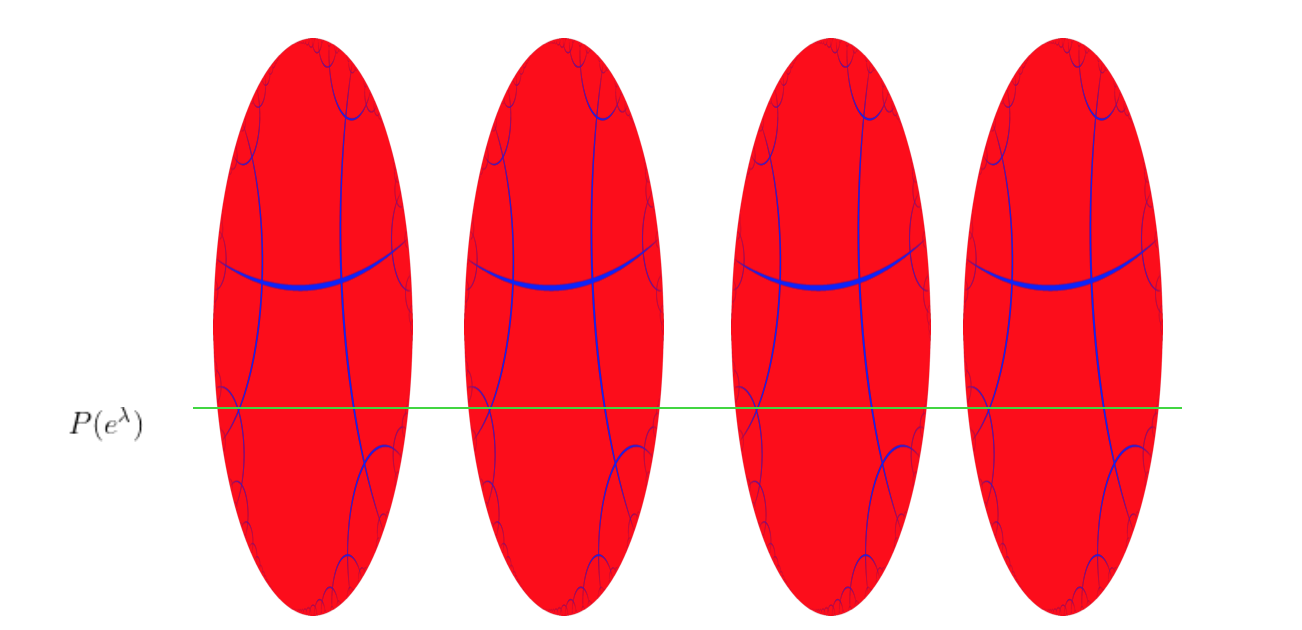
\includegraphics{images/tube}}
\end{figure}
\end{frame}

\begin{frame}[fragile]
\frametitle{Flow}
\begin{itemize}
    \item Function as flow
    \item Integral as flow
    \item Limited process as flow
\end{itemize}
\begin{columns}
\begin{column}{0.5\textwidth}
\begin{center}
    \begin{tikzcd}
        H && H \\
        R && R
        \arrow["l", from=1-1, to=1-3]
        \arrow["\nu"', from=1-1, to=2-1]
        \arrow["\nu", from=1-3, to=2-3]
        \arrow["k"', from=2-1, to=2-3]
    \end{tikzcd}
\end{center}
\end{column}
\begin{column}{0.5\textwidth}
    \begin{figure}[ht]\centering
    \resizebox{\textwidth}{!}{
\includegraphics{images/flow}}
    \end{figure}
\end{column}
\end{columns}
\end{frame}

\begin{frame}
\frametitle{Extend calculus by mixing addition and multiplication?}
    Riemann sum is purely additional.
    Can we extend it by mixing addition and multiplication?
\end{frame}

\begin{frame}
\frametitle{Calculus as a boundary algebra?}
    Infinitely small values and large values are appeared at the boundary.
    Limitation process can be treated as flow to the boundary.
\begin{figure}[ht]\centering
\resizebox{0.4\textwidth}{!}{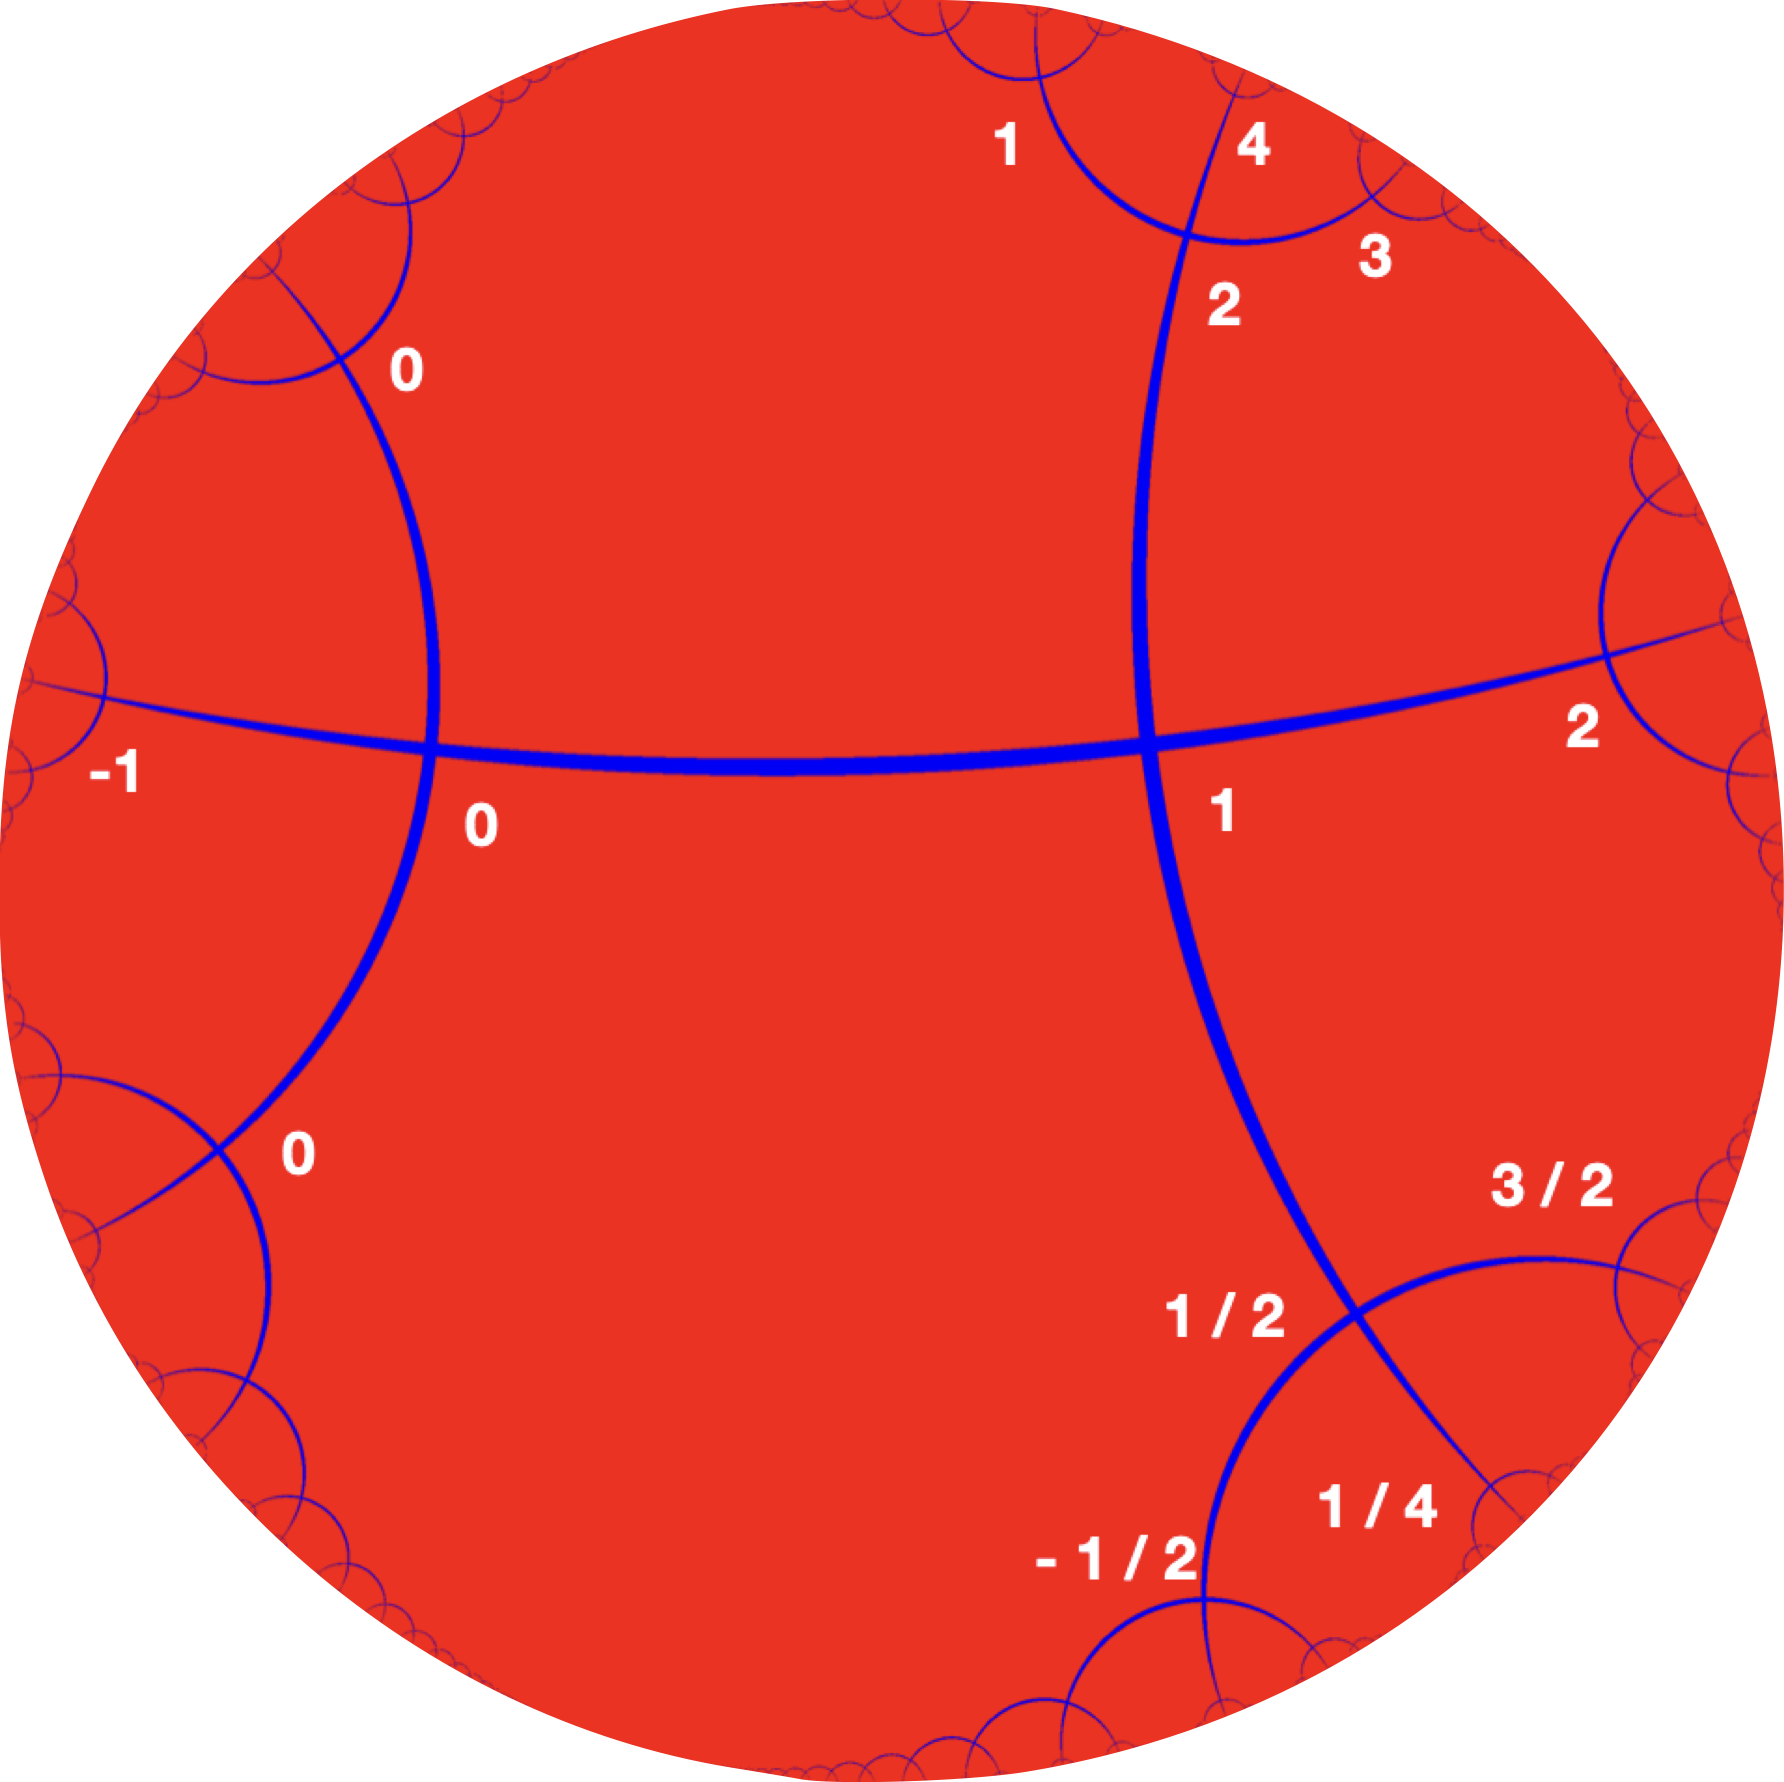
\includegraphics{images/assignment2}}
\end{figure}
\end{frame}

\begin{frame}
\frametitle{Other analysis systems?}
    Formulate our systems as a tuple of
    \begin{itemize}
        \item $E(F), (H, a), (Path, Integ)$
    \end{itemize}
    Here we have
    \begin{itemize}
        \item $E(F)$: Expressions over a field $F$
        \item $(H, a)$: A scalar field "assignment" $a$ on a space $H$
        \item $(Path, Integ)$: all paths can be interpreted as an integral
    \end{itemize}
    Can we form a category? and complex analysis is an example?
\end{frame}

\section{Adventure in a wonderland}

\begin{frame}
\frametitle{Adventure in a wonderland}
\begin{figure}[ht]\centering
\resizebox{0.5\textwidth}{!}{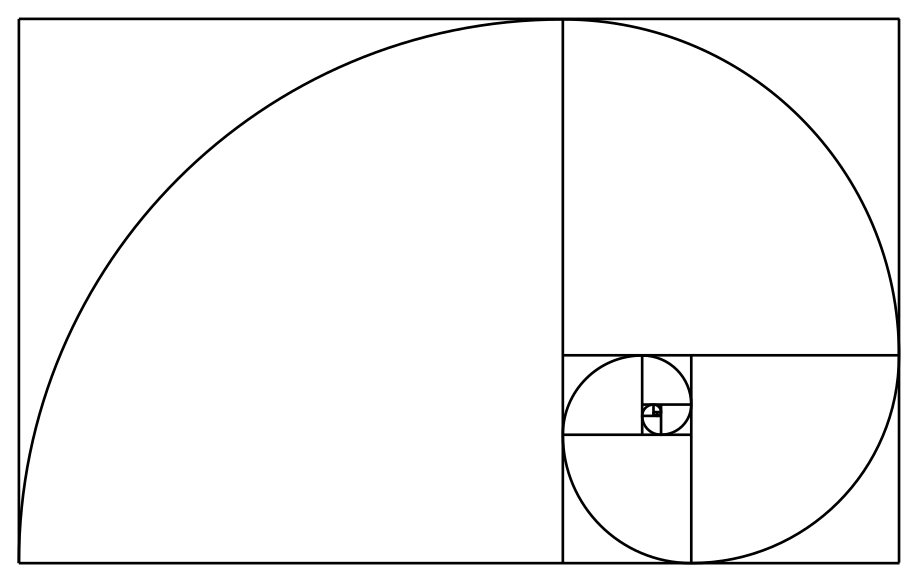
\includegraphics{images/fibonacci_spiral.png}}
\end{figure}
\end{frame}

\begin{frame}
\frametitle{SKI combinator calculus}
\begin{columns}
\begin{column}{0.5\textwidth}
    \begin{figure}[ht]\centering
    \resizebox{0.8\textwidth}{!}{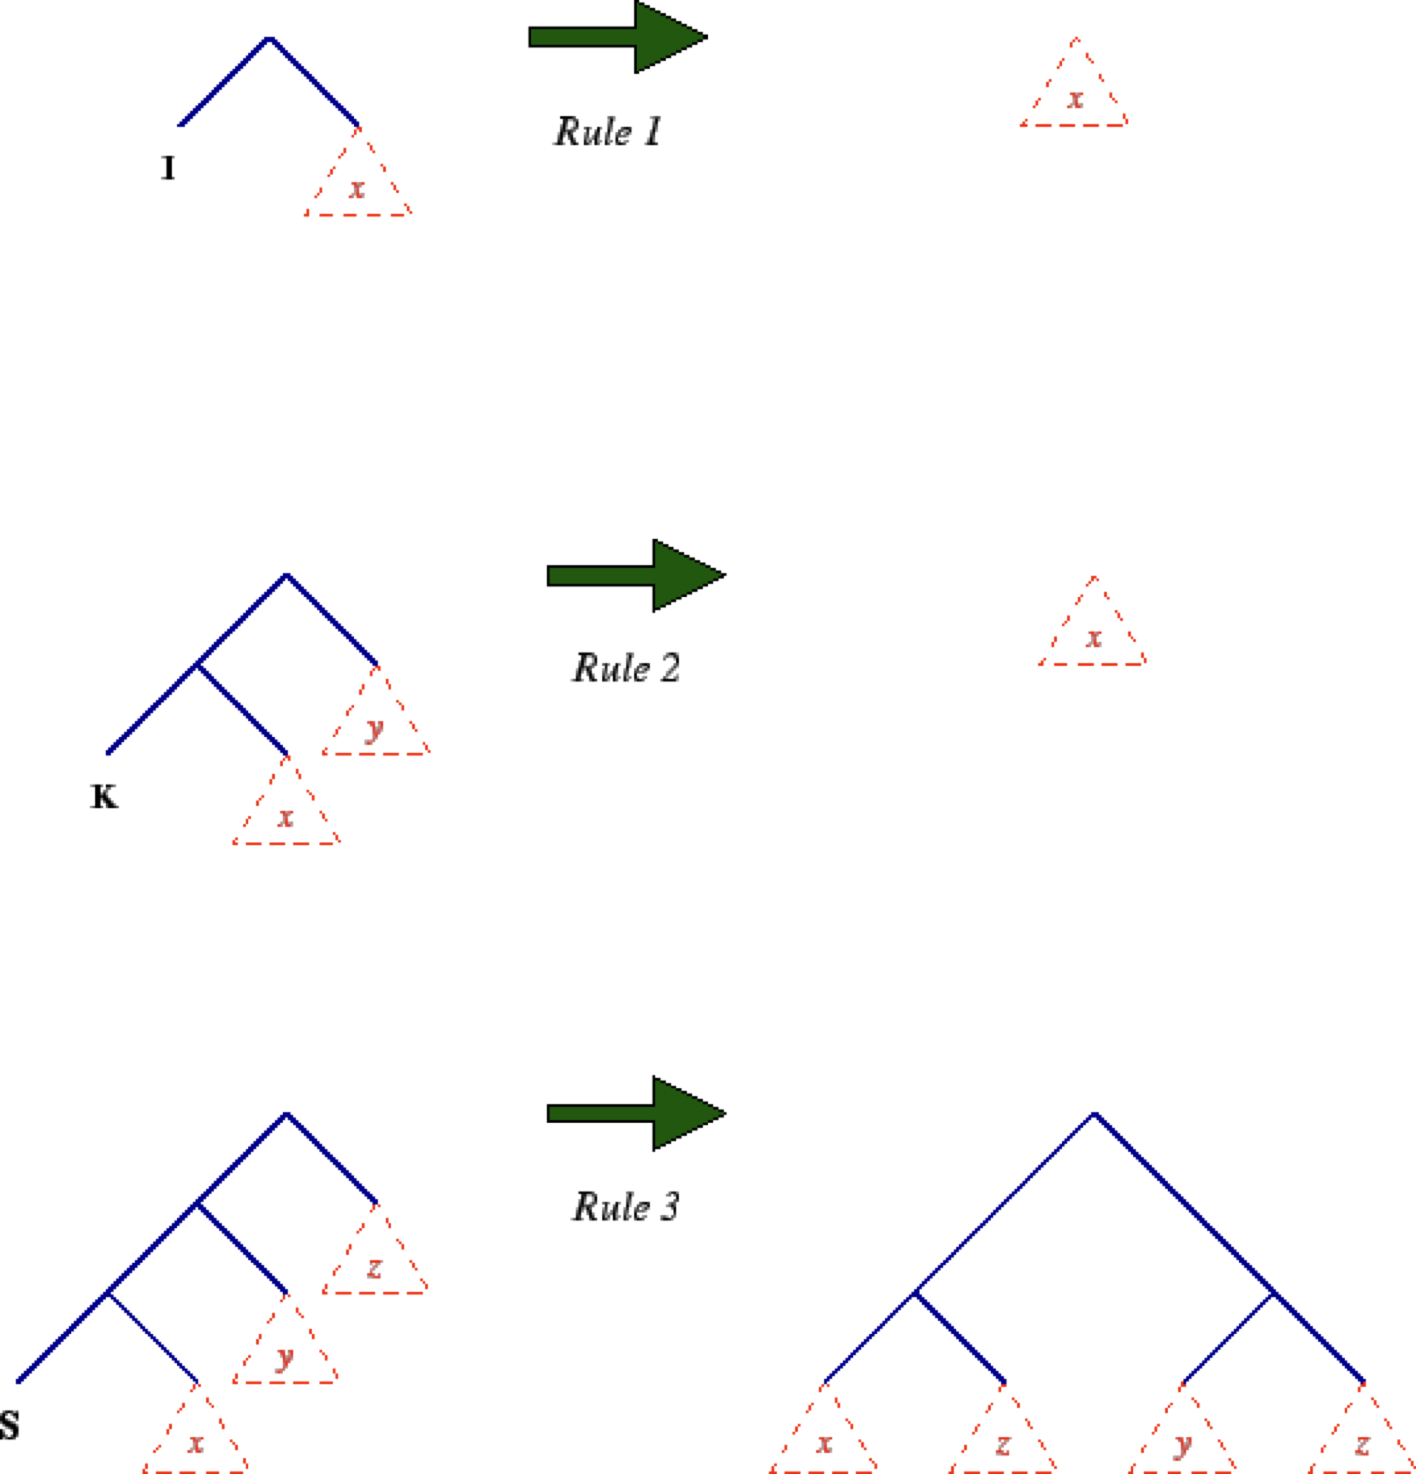
\includegraphics{images/ski-rules.png}}
    \end{figure}
\end{column}
\begin{column}{0.5\textwidth}
    \begin{figure}[ht]\centering
    \resizebox{0.8\textwidth}{!}{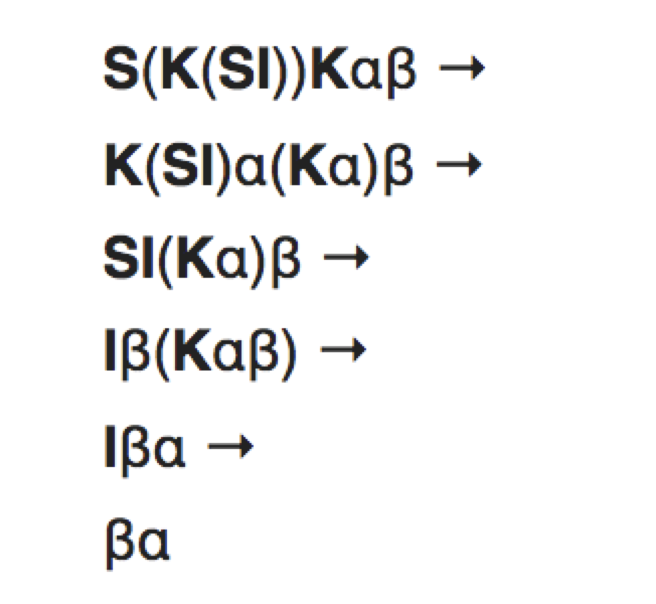
\includegraphics{images/ski-reverse.png}}
    \end{figure}
\end{column}
\end{columns}
\end{frame}

\begin{frame}
\frametitle{A space of SKI combinators}
    Any arithmetic expression can be represented by SKI combinators via Church numerals.
    So any arithmetic expression space can be encoded by SKI combinators.

    Program space!
\end{frame}

\begin{frame}
\frametitle{Ancient Egyptian multiplication}
    \begin{figure}[ht]\centering
    \resizebox{0.8\textwidth}{!}{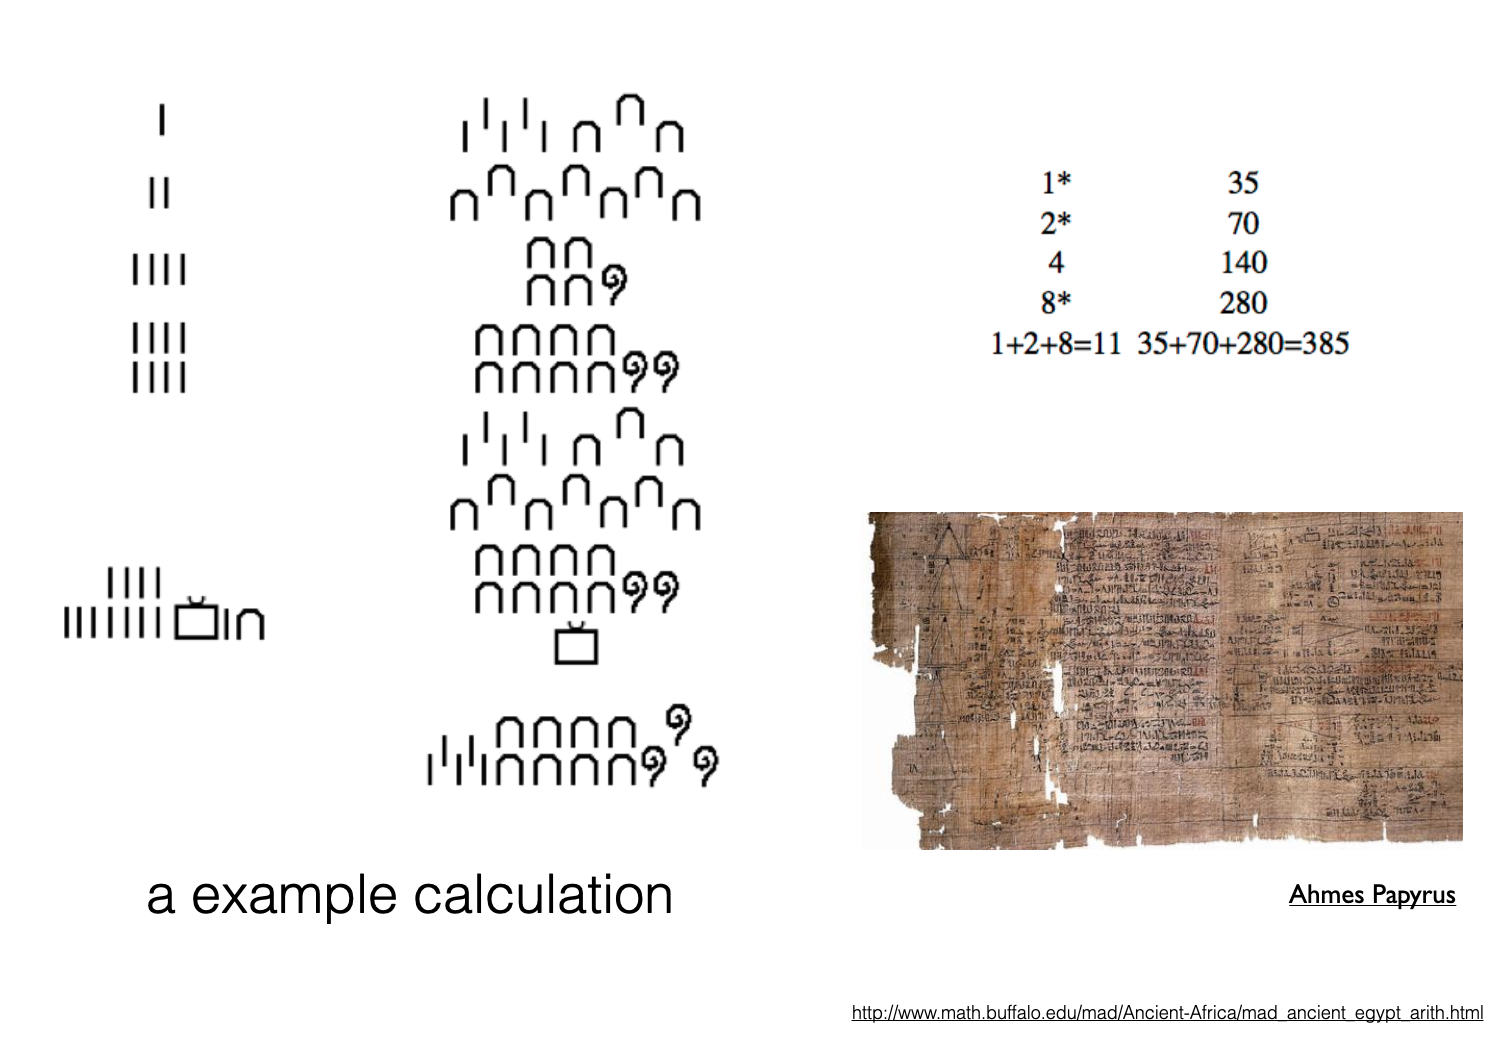
\includegraphics{images/egyptian.png}}
    \end{figure}
\end{frame}

\begin{frame}
\frametitle{A story of square root of 17}
A story from Plato's Theaetetus: Theodorus of Cyrene, a young mathematician, was able to prove that $\sqrt{3}$, $\sqrt{5}$... are irrational, but not $\sqrt{17}$.

\begin{columns}
\begin{column}{0.5\textwidth}
    \begin{figure}[ht]\centering
    \resizebox{0.6\textwidth}{!}{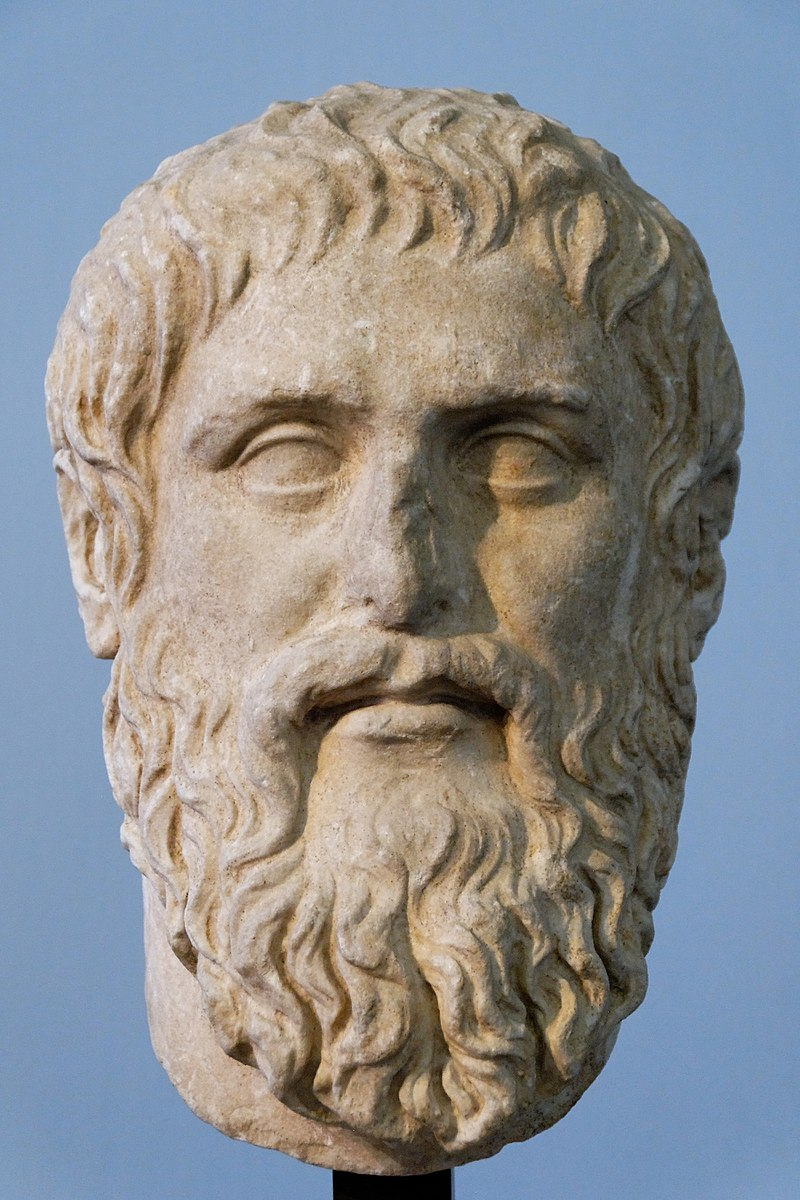
\includegraphics{images/Plato.jpeg}}
    \end{figure}
\end{column}
\begin{column}{0.5\textwidth}
    \begin{figure}[ht]\centering
    \resizebox{0.8\textwidth}{!}{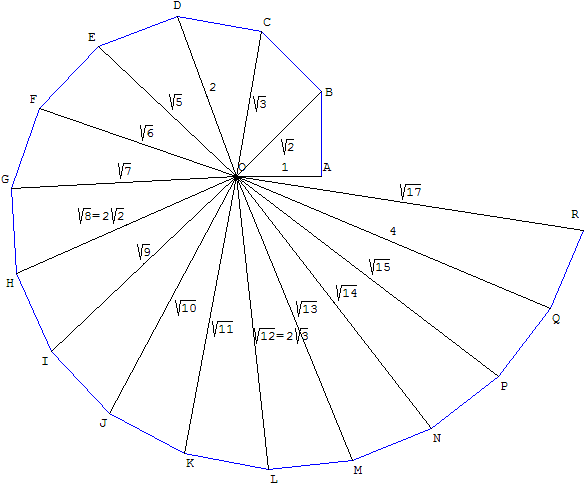
\includegraphics{images/escargot_pythagore.png}}
    \end{figure}
\end{column}
\end{columns}
\end{frame}

\begin{frame}
\frametitle{A logic system as a space?}
The axioms by Victor Pambuccian and Celia Schacht are also fit into expressions,
and then some terms of the system can be embedded into the expression space.
Can we migrate the problem of irrationality of $\sqrt{17}$ from proof theory into a problem in group theory?
\begin{columns}
\begin{column}{0.4\textwidth}
    \begin{figure}[ht]\centering
    \resizebox{0.8\textwidth}{!}{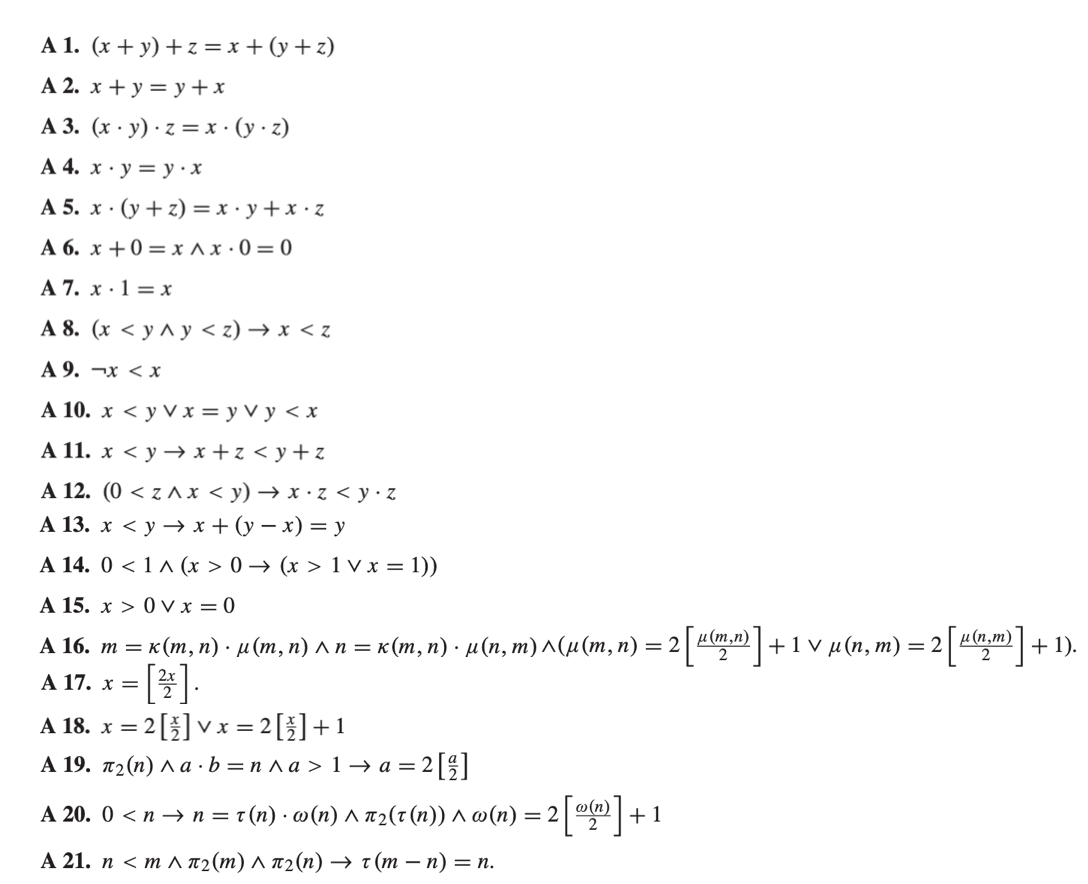
\includegraphics{images/axioms.png}}
    \end{figure}
\end{column}
\begin{column}{0.4\textwidth}
\begin{figure}[ht]
\centering

\tikzmath{
  \one = 1;
  \base = 2;
  \offset = 15.8888888;
  \valofpi = 3.1415926;
  \anglei = 3.1415926;
  \angleo = 3.1415926;
}

\resizebox{0.8\columnwidth}{!}{%
\begin{tikzpicture}
\draw [black, line width=0.6pt, ->] (15.875,0) to[out=90,in=270] (15.875,33);
\node [anchor=south] at (16,33) {y};
\draw [black, line width=0.6pt, ->] (-16.5,0) to[out=0,in=180] (18,0);
\node [anchor=west] at (18.5,0) {x};

\foreach \x in {-35,...,2}
  \node [anchor=north] at (\x / 9 * 8 + \offset,0) {\x};
\foreach \y in {1,...,36}
  \node [anchor=-135] at (18,\y / 9 * 8) {\y};

\foreach \t in {36, ..., 1}
  \draw [lightgray, line width=0.6pt] (-16.5, \t / 9 * 8) to[out=0,in=180] (18, \t / 9 * 8);

\foreach \t in {-36, ..., 2}
  \draw [lightgray, line width=0.6pt] (\t / 9 * 8 + \offset, 0) to[out=90,in=270] (\t / 9 * 8 + \offset, 33);

\draw [green, line width=1.0pt] (-36 / 9 * 8 + \offset, 0) to[out=90,in=270] (-36 / 9 * 8 + \offset, 4 / 9 * 8);
\draw [green, line width=1.0pt] (-35 / 9 * 8 + \offset, 0) to[out=90,in=270] (-35 / 9 * 8 + \offset, 1 / 9 * 8);
\draw [green, line width=1.0pt] (-34 / 9 * 8 + \offset, 0) to[out=90,in=270] (-34 / 9 * 8 + \offset, 2 / 9 * 8);
\draw [green, line width=1.0pt] (-33 / 9 * 8 + \offset, 0) to[out=90,in=270] (-33 / 9 * 8 + \offset, 1 / 9 * 8);
\draw [green, line width=1.0pt] (-32 / 9 * 8 + \offset, 0) to[out=90,in=270] (-32 / 9 * 8 + \offset, 32 / 9 * 8);
\draw [green, line width=1.0pt] (-31 / 9 * 8 + \offset, 0) to[out=90,in=270] (-31 / 9 * 8 + \offset, 1 / 9 * 8);
\draw [green, line width=1.0pt] (-30 / 9 * 8 + \offset, 0) to[out=90,in=270] (-30 / 9 * 8 + \offset, 2 / 9 * 8);
\draw [green, line width=1.0pt] (-29 / 9 * 8 + \offset, 0) to[out=90,in=270] (-29 / 9 * 8 + \offset, 1 / 9 * 8);
\draw [green, line width=1.0pt] (-28 / 9 * 8 + \offset, 0) to[out=90,in=270] (-28 / 9 * 8 + \offset, 4 / 9 * 8);
\draw [green, line width=1.0pt] (-27 / 9 * 8 + \offset, 0) to[out=90,in=270] (-27 / 9 * 8 + \offset, 1 / 9 * 8);
\draw [green, line width=1.0pt] (-26 / 9 * 8 + \offset, 0) to[out=90,in=270] (-26 / 9 * 8 + \offset, 2 / 9 * 8);
\draw [green, line width=1.0pt] (-25 / 9 * 8 + \offset, 0) to[out=90,in=270] (-25 / 9 * 8 + \offset, 1 / 9 * 8);
\draw [green, line width=1.0pt] (-24 / 9 * 8 + \offset, 0) to[out=90,in=270] (-24 / 9 * 8 + \offset, 8 / 9 * 8);
\draw [green, line width=1.0pt] (-23 / 9 * 8 + \offset, 0) to[out=90,in=270] (-23 / 9 * 8 + \offset, 1 / 9 * 8);
\draw [green, line width=1.0pt] (-22 / 9 * 8 + \offset, 0) to[out=90,in=270] (-22 / 9 * 8 + \offset, 2 / 9 * 8);
\draw [green, line width=1.0pt] (-21 / 9 * 8 + \offset, 0) to[out=90,in=270] (-21 / 9 * 8 + \offset, 1 / 9 * 8);
\draw [green, line width=1.0pt] (-20 / 9 * 8 + \offset, 0) to[out=90,in=270] (-20 / 9 * 8 + \offset, 4 / 9 * 8);
\draw [green, line width=1.0pt] (-19 / 9 * 8 + \offset, 0) to[out=90,in=270] (-19 / 9 * 8 + \offset, 1 / 9 * 8);
\draw [green, line width=1.0pt] (-18 / 9 * 8 + \offset, 0) to[out=90,in=270] (-18 / 9 * 8 + \offset, 2 / 9 * 8);
\draw [green, line width=1.0pt] (-17 / 9 * 8 + \offset, 0) to[out=90,in=270] (-17 / 9 * 8 + \offset, 1 / 9 * 8);
\draw [green, line width=1.0pt] (-16 / 9 * 8 + \offset, 0) to[out=90,in=270] (-16 / 9 * 8 + \offset, 16 / 9 * 8);
\draw [green, line width=1.0pt] (-15 / 9 * 8 + \offset, 0) to[out=90,in=270] (-15 / 9 * 8 + \offset, 1 / 9 * 8);
\draw [green, line width=1.0pt] (-14 / 9 * 8 + \offset, 0) to[out=90,in=270] (-14 / 9 * 8 + \offset, 2 / 9 * 8);
\draw [green, line width=1.0pt] (-13 / 9 * 8 + \offset, 0) to[out=90,in=270] (-13 / 9 * 8 + \offset, 1 / 9 * 8);
\draw [green, line width=1.0pt] (-12 / 9 * 8 + \offset, 0) to[out=90,in=270] (-12 / 9 * 8 + \offset, 4 / 9 * 8);
\draw [green, line width=1.0pt] (-11 / 9 * 8 + \offset, 0) to[out=90,in=270] (-11 / 9 * 8 + \offset, 1 / 9 * 8);
\draw [green, line width=1.0pt] (-10 / 9 * 8 + \offset, 0) to[out=90,in=270] (-10 / 9 * 8 + \offset, 2 / 9 * 8);
\draw [green, line width=1.0pt] (-9 / 9 * 8 + \offset, 0) to[out=90,in=270] (-9 / 9 * 8 + \offset, 1 / 9 * 8);
\draw [green, line width=1.0pt] (-8 / 9 * 8 + \offset, 0) to[out=90,in=270] (-8 / 9 * 8 + \offset, 8 / 9 * 8);
\draw [green, line width=1.0pt] (-7 / 9 * 8 + \offset, 0) to[out=90,in=270] (-7 / 9 * 8 + \offset, 1 / 9 * 8);
\draw [green, line width=1.0pt] (-6 / 9 * 8 + \offset, 0) to[out=90,in=270] (-6 / 9 * 8 + \offset, 2 / 9 * 8);
\draw [green, line width=1.0pt] (-5 / 9 * 8 + \offset, 0) to[out=90,in=270] (-5 / 9 * 8 + \offset, 1 / 9 * 8);
\draw [green, line width=1.0pt] (-4 / 9 * 8 + \offset, 0) to[out=90,in=270] (-4 / 9 * 8 + \offset, 4 / 9 * 8);
\draw [green, line width=1.0pt] (-3 / 9 * 8 + \offset, 0) to[out=90,in=270] (-3 / 9 * 8 + \offset, 1 / 9 * 8);
\draw [green, line width=1.0pt] (-2 / 9 * 8 + \offset, 0) to[out=90,in=270] (-2 / 9 * 8 + \offset, 2 / 9 * 8);
\draw [green, line width=1.0pt] (-1 / 9 * 8 + \offset, 0) to[out=90,in=270] (-1 / 9 * 8 + \offset, 1 / 9 * 8);

\foreach \a in {32, 16, 8, 4, 2, 1}
    \draw [blue, line width=0.6pt] (-16.5, \a / 9 * 8) to[out=0,in=180] (18, \a / 9 * 8);

\node[circle,fill=black,inner sep=1pt,minimum size=3pt] (a) at (-32 / 9 * 8 + \offset, 32 / 9 * 8) {};
\node [anchor=315, red] at (-32 / 9 * 8 + \offset, 32 / 9 * 8) {1};

\node[circle,fill=black,inner sep=1pt,minimum size=3pt] (a) at (-16 / 9 * 8 + \offset, 16 / 9 * 8) {};
\node [anchor=315, red] at (-16 / 9 * 8 + \offset, 16 / 9 * 8) {1};
\node[circle,fill=black,inner sep=1pt,minimum size=3pt] (a) at (-16 / 9 * 8 + \offset, 16 / 9 * 8) {};
\node [anchor=315, red] at (-32 / 9 * 8 + \offset, 16 / 9 * 8) {2};

\node[circle,fill=black,inner sep=1pt,minimum size=3pt] (b) at (-8 / 9 * 8 + \offset, 8 / 9 * 8) {};
\node [anchor=315, red] at (-8 / 9 * 8 + \offset, 8 / 9 * 8) {1};
\node[circle,fill=black,inner sep=1pt,minimum size=3pt] (b) at (-16 / 9 * 8 + \offset, 8 / 9 * 8) {};
\node [anchor=315, red] at (-16 / 9 * 8 + \offset, 8 / 9 * 8) {2};
\node[circle,fill=black,inner sep=1pt,minimum size=3pt] (b) at (-16 / 9 * 8 + \offset, 8 / 9 * 8) {};
\node [anchor=315, red] at (-24 / 9 * 8 + \offset, 8 / 9 * 8) {3};
\node[circle,fill=black,inner sep=1pt,minimum size=3pt] (b) at (-16 / 9 * 8 + \offset, 8 / 9 * 8) {};
\node [anchor=315, red] at (-32 / 9 * 8 + \offset, 8 / 9 * 8) {4};

\node[circle,fill=black,inner sep=1pt,minimum size=3pt] (b) at (-4 / 9 * 8 + \offset, 4 / 9 * 8) {};
\node [anchor=315, red] at (-4 / 9 * 8 + \offset, 4 / 9 * 8) {1};
\node[circle,fill=black,inner sep=1pt,minimum size=3pt] (b) at (-8 / 9 * 8 + \offset, 4 / 9 * 8) {};
\node [anchor=315, red] at (-8 / 9 * 8 + \offset, 4 / 9 * 8) {2};
\node[circle,fill=black,inner sep=1pt,minimum size=3pt] (b) at (-12 / 9 * 8 + \offset, 4 / 9 * 8) {};
\node [anchor=315, red] at (-12 / 9 * 8 + \offset, 4 / 9 * 8) {3};
\node[circle,fill=black,inner sep=1pt,minimum size=3pt] (b) at (-16 / 9 * 8 + \offset, 4 / 9 * 8) {};
\node [anchor=315, red] at (-16 / 9 * 8 + \offset, 4 / 9 * 8) {4};
\node[circle,fill=black,inner sep=1pt,minimum size=3pt] (b) at (-20 / 9 * 8 + \offset, 4 / 9 * 8) {};
\node [anchor=315, red] at (-20 / 9 * 8 + \offset, 4 / 9 * 8) {5};
\node[circle,fill=black,inner sep=1pt,minimum size=3pt] (b) at (-24 / 9 * 8 + \offset, 4 / 9 * 8) {};
\node [anchor=315, red] at (-24 / 9 * 8 + \offset, 4 / 9 * 8) {6};
\node[circle,fill=black,inner sep=1pt,minimum size=3pt] (b) at (-28 / 9 * 8 + \offset, 4 / 9 * 8) {};
\node [anchor=315, red] at (-28 / 9 * 8 + \offset, 4 / 9 * 8) {7};
\node[circle,fill=black,inner sep=1pt,minimum size=3pt] (b) at (-32 / 9 * 8 + \offset, 4 / 9 * 8) {};
\node [anchor=315, red] at (-32 / 9 * 8 + \offset, 4 / 9 * 8) {8};
\node[circle,fill=black,inner sep=1pt,minimum size=3pt] (b) at (-36 / 9 * 8 + \offset, 4 / 9 * 8) {};
\node [anchor=315, red] at (-36 / 9 * 8 + \offset, 4 / 9 * 8) {9};

\node[circle,fill=black,inner sep=1pt,minimum size=3pt] (b) at (-2 / 9 * 8 + \offset, 2 / 9 * 8) {};
\node [anchor=315, red] at (-2 / 9 * 8 + \offset, 2 / 9 * 8) {1};
\node[circle,fill=black,inner sep=1pt,minimum size=3pt] (b) at (-4 / 9 * 8 + \offset, 2 / 9 * 8) {};
\node [anchor=315, red] at (-4 / 9 * 8 + \offset, 2 / 9 * 8) {2};
\node[circle,fill=black,inner sep=1pt,minimum size=3pt] (b) at (-6 / 9 * 8 + \offset, 2 / 9 * 8) {};
\node [anchor=315, red] at (-6 / 9 * 8 + \offset, 2 / 9 * 8) {3};
\node[circle,fill=black,inner sep=1pt,minimum size=3pt] (b) at (-8 / 9 * 8 + \offset, 2 / 9 * 8) {};
\node [anchor=315, red] at (-8 / 9 * 8 + \offset, 2 / 9 * 8) {4};
\node[circle,fill=black,inner sep=1pt,minimum size=3pt] (b) at (-10 / 9 * 8 + \offset, 2 / 9 * 8) {};
\node [anchor=315, red] at (-10 / 9 * 8 + \offset, 2 / 9 * 8) {5};
\node[circle,fill=black,inner sep=1pt,minimum size=3pt] (b) at (-12 / 9 * 8 + \offset, 2 / 9 * 8) {};
\node [anchor=315, red] at (-12 / 9 * 8 + \offset, 2 / 9 * 8) {6};
\node[circle,fill=black,inner sep=1pt,minimum size=3pt] (b) at (-14 / 9 * 8 + \offset, 2 / 9 * 8) {};
\node [anchor=315, red] at (-14 / 9 * 8 + \offset, 2 / 9 * 8) {7};
\node[circle,fill=black,inner sep=1pt,minimum size=3pt] (b) at (-16 / 9 * 8 + \offset, 2 / 9 * 8) {};
\node [anchor=315, red] at (-16 / 9 * 8 + \offset, 2 / 9 * 8) {8};
\node[circle,fill=black,inner sep=1pt,minimum size=3pt] (b) at (-18 / 9 * 8 + \offset, 2 / 9 * 8) {};
\node [anchor=315, red] at (-18 / 9 * 8 + \offset, 2 / 9 * 8) {9};
\node[circle,fill=black,inner sep=1pt,minimum size=3pt] (b) at (-20 / 9 * 8 + \offset, 2 / 9 * 8) {};
\node [anchor=315, red] at (-20 / 9 * 8 + \offset, 2 / 9 * 8) {10};
\node[circle,fill=black,inner sep=1pt,minimum size=3pt] (b) at (-22 / 9 * 8 + \offset, 2 / 9 * 8) {};
\node [anchor=315, red] at (-22 / 9 * 8 + \offset, 2 / 9 * 8) {11};
\node[circle,fill=black,inner sep=1pt,minimum size=3pt] (b) at (-24 / 9 * 8 + \offset, 2 / 9 * 8) {};
\node [anchor=315, red] at (-24 / 9 * 8 + \offset, 2 / 9 * 8) {12};
\node[circle,fill=black,inner sep=1pt,minimum size=3pt] (b) at (-26 / 9 * 8 + \offset, 2 / 9 * 8) {};
\node [anchor=315, red] at (-26 / 9 * 8 + \offset, 2 / 9 * 8) {13};
\node[circle,fill=black,inner sep=1pt,minimum size=3pt] (b) at (-28 / 9 * 8 + \offset, 2 / 9 * 8) {};
\node [anchor=315, red] at (-28 / 9 * 8 + \offset, 2 / 9 * 8) {14};
\node[circle,fill=black,inner sep=1pt,minimum size=3pt] (b) at (-30 / 9 * 8 + \offset, 2 / 9 * 8) {};
\node [anchor=315, red] at (-30 / 9 * 8 + \offset, 2 / 9 * 8) {15};
\node[circle,fill=black,inner sep=1pt,minimum size=3pt] (b) at (-32 / 9 * 8 + \offset, 2 / 9 * 8) {};
\node [anchor=315, red] at (-32 / 9 * 8 + \offset, 2 / 9 * 8) {16};
\node[circle,fill=black,inner sep=1pt,minimum size=3pt] (b) at (-34 / 9 * 8 + \offset, 2 / 9 * 8) {};
\node [anchor=315, red] at (-34 / 9 * 8 + \offset, 2 / 9 * 8) {17};
\node[circle,fill=black,inner sep=1pt,minimum size=3pt] (b) at (-36 / 9 * 8 + \offset, 2 / 9 * 8) {};
\node [anchor=315, red] at (-36 / 9 * 8 + \offset, 2 / 9 * 8) {18};

\node[circle,fill=black,inner sep=1pt,minimum size=3pt] (b) at (-1 / 9 * 8 + \offset, 1 / 9 * 8) {};
\node [anchor=315, red] at (-1 / 9 * 8 + \offset, 1 / 9 * 8) {1};
\node[circle,fill=black,inner sep=1pt,minimum size=3pt] (b) at (-2 / 9 * 8 + \offset, 1 / 9 * 8) {};
\node [anchor=315, red] at (-2 / 9 * 8 + \offset, 1 / 9 * 8) {2};
\node[circle,fill=black,inner sep=1pt,minimum size=3pt] (b) at (-3 / 9 * 8 + \offset, 1 / 9 * 8) {};
\node [anchor=315, red] at (-3 / 9 * 8 + \offset, 1 / 9 * 8) {3};
\node[circle,fill=black,inner sep=1pt,minimum size=3pt] (b) at (-4 / 9 * 8 + \offset, 1 / 9 * 8) {};
\node [anchor=315, red] at (-4 / 9 * 8 + \offset, 1 / 9 * 8) {4};
\node[circle,fill=black,inner sep=1pt,minimum size=3pt] (b) at (-5 / 9 * 8 + \offset, 1 / 9 * 8) {};
\node [anchor=315, red] at (-5 / 9 * 8 + \offset, 1 / 9 * 8) {5};
\node[circle,fill=black,inner sep=1pt,minimum size=3pt] (b) at (-6 / 9 * 8 + \offset, 1 / 9 * 8) {};
\node [anchor=315, red] at (-6 / 9 * 8 + \offset, 1 / 9 * 8) {6};
\node[circle,fill=black,inner sep=1pt,minimum size=3pt] (b) at (-7 / 9 * 8 + \offset, 1 / 9 * 8) {};
\node [anchor=315, red] at (-7 / 9 * 8 + \offset, 1 / 9 * 8) {7};
\node[circle,fill=black,inner sep=1pt,minimum size=3pt] (b) at (-8 / 9 * 8 + \offset, 1 / 9 * 8) {};
\node [anchor=315, red] at (-8 / 9 * 8 + \offset, 1 / 9 * 8) {8};
\node[circle,fill=black,inner sep=1pt,minimum size=3pt] (b) at (-9 / 9 * 8 + \offset, 1 / 9 * 8) {};
\node [anchor=315, red] at (-9 / 9 * 8 + \offset, 1 / 9 * 8) {9};
\node[circle,fill=black,inner sep=1pt,minimum size=3pt] (b) at (-10 / 9 * 8 + \offset, 1 / 9 * 8) {};
\node [anchor=315, red] at (-10 / 9 * 8 + \offset, 1 / 9 * 8) {10};
\node[circle,fill=black,inner sep=1pt,minimum size=3pt] (b) at (-11 / 9 * 8 + \offset, 1 / 9 * 8) {};
\node [anchor=315, red] at (-11 / 9 * 8 + \offset, 1 / 9 * 8) {11};
\node[circle,fill=black,inner sep=1pt,minimum size=3pt] (b) at (-12 / 9 * 8 + \offset, 1 / 9 * 8) {};
\node [anchor=315, red] at (-12 / 9 * 8 + \offset, 1 / 9 * 8) {12};
\node[circle,fill=black,inner sep=1pt,minimum size=3pt] (b) at (-13 / 9 * 8 + \offset, 1 / 9 * 8) {};
\node [anchor=315, red] at (-13 / 9 * 8 + \offset, 1 / 9 * 8) {13};
\node[circle,fill=black,inner sep=1pt,minimum size=3pt] (b) at (-14 / 9 * 8 + \offset, 1 / 9 * 8) {};
\node [anchor=315, red] at (-14 / 9 * 8 + \offset, 1 / 9 * 8) {14};
\node[circle,fill=black,inner sep=1pt,minimum size=3pt] (b) at (-15 / 9 * 8 + \offset, 1 / 9 * 8) {};
\node [anchor=315, red] at (-15 / 9 * 8 + \offset, 1 / 9 * 8) {15};
\node[circle,fill=black,inner sep=1pt,minimum size=3pt] (b) at (-16 / 9 * 8 + \offset, 1 / 9 * 8) {};
\node [anchor=315, red] at (-16 / 9 * 8 + \offset, 1 / 9 * 8) {16};
\node[circle,fill=black,inner sep=1pt,minimum size=3pt] (b) at (-17 / 9 * 8 + \offset, 1 / 9 * 8) {};
\node [anchor=315, red] at (-17 / 9 * 8 + \offset, 1 / 9 * 8) {17};
\node[circle,fill=black,inner sep=1pt,minimum size=3pt] (b) at (-18 / 9 * 8 + \offset, 1 / 9 * 8) {};
\node [anchor=315, red] at (-18 / 9 * 8 + \offset, 1 / 9 * 8) {18};
\node[circle,fill=black,inner sep=1pt,minimum size=3pt] (b) at (-19 / 9 * 8 + \offset, 1 / 9 * 8) {};
\node [anchor=315, red] at (-19 / 9 * 8 + \offset, 1 / 9 * 8) {19};
\node[circle,fill=black,inner sep=1pt,minimum size=3pt] (b) at (-20 / 9 * 8 + \offset, 1 / 9 * 8) {};
\node [anchor=315, red] at (-20 / 9 * 8 + \offset, 1 / 9 * 8) {20};
\node[circle,fill=black,inner sep=1pt,minimum size=3pt] (b) at (-21 / 9 * 8 + \offset, 1 / 9 * 8) {};
\node [anchor=315, red] at (-21 / 9 * 8 + \offset, 1 / 9 * 8) {21};
\node[circle,fill=black,inner sep=1pt,minimum size=3pt] (b) at (-22 / 9 * 8 + \offset, 1 / 9 * 8) {};
\node [anchor=315, red] at (-22 / 9 * 8 + \offset, 1 / 9 * 8) {22};
\node[circle,fill=black,inner sep=1pt,minimum size=3pt] (b) at (-23 / 9 * 8 + \offset, 1 / 9 * 8) {};
\node [anchor=315, red] at (-23 / 9 * 8 + \offset, 1 / 9 * 8) {23};
\node[circle,fill=black,inner sep=1pt,minimum size=3pt] (b) at (-24 / 9 * 8 + \offset, 1 / 9 * 8) {};
\node [anchor=315, red] at (-24 / 9 * 8 + \offset, 1 / 9 * 8) {24};
\node[circle,fill=black,inner sep=1pt,minimum size=3pt] (b) at (-25 / 9 * 8 + \offset, 1 / 9 * 8) {};
\node [anchor=315, red] at (-25 / 9 * 8 + \offset, 1 / 9 * 8) {25};
\node[circle,fill=black,inner sep=1pt,minimum size=3pt] (b) at (-26 / 9 * 8 + \offset, 1 / 9 * 8) {};
\node [anchor=315, red] at (-26 / 9 * 8 + \offset, 1 / 9 * 8) {26};
\node[circle,fill=black,inner sep=1pt,minimum size=3pt] (b) at (-27 / 9 * 8 + \offset, 1 / 9 * 8) {};
\node [anchor=315, red] at (-27 / 9 * 8 + \offset, 1 / 9 * 8) {27};
\node[circle,fill=black,inner sep=1pt,minimum size=3pt] (b) at (-28 / 9 * 8 + \offset, 1 / 9 * 8) {};
\node [anchor=315, red] at (-28 / 9 * 8 + \offset, 1 / 9 * 8) {28};
\node[circle,fill=black,inner sep=1pt,minimum size=3pt] (b) at (-29 / 9 * 8 + \offset, 1 / 9 * 8) {};
\node [anchor=315, red] at (-29 / 9 * 8 + \offset, 1 / 9 * 8) {29};
\node[circle,fill=black,inner sep=1pt,minimum size=3pt] (b) at (-30 / 9 * 8 + \offset, 1 / 9 * 8) {};
\node [anchor=315, red] at (-30 / 9 * 8 + \offset, 1 / 9 * 8) {30};
\node[circle,fill=black,inner sep=1pt,minimum size=3pt] (b) at (-31 / 9 * 8 + \offset, 1 / 9 * 8) {};
\node [anchor=315, red] at (-31 / 9 * 8 + \offset, 1 / 9 * 8) {31};
\node[circle,fill=black,inner sep=1pt,minimum size=3pt] (b) at (-32 / 9 * 8 + \offset, 1 / 9 * 8) {};
\node [anchor=315, red] at (-32 / 9 * 8 + \offset, 1 / 9 * 8) {32};
\node[circle,fill=black,inner sep=1pt,minimum size=3pt] (b) at (-33 / 9 * 8 + \offset, 1 / 9 * 8) {};
\node [anchor=315, red] at (-33 / 9 * 8 + \offset, 1 / 9 * 8) {33};
\node[circle,fill=black,inner sep=1pt,minimum size=3pt] (b) at (-34 / 9 * 8 + \offset, 1 / 9 * 8) {};
\node [anchor=315, red] at (-34 / 9 * 8 + \offset, 1 / 9 * 8) {34};
\node[circle,fill=black,inner sep=1pt,minimum size=3pt] (b) at (-35 / 9 * 8 + \offset, 1 / 9 * 8) {};
\node [anchor=315, red] at (-35 / 9 * 8 + \offset, 1 / 9 * 8) {35};
\node[circle,fill=black,inner sep=1pt,minimum size=3pt] (b) at (-36 / 9 * 8 + \offset, 1 / 9 * 8) {};
\node [anchor=315, red] at (-36 / 9 * 8 + \offset, 1 / 9 * 8) {36};

\draw [brown, line width=1.0pt] (1 / 9 * 8 + \offset, 3 / 9 * 8) to[out=251.5651,in=71.5651] (0 / 9 * 8 + \offset, 0 / 9 * 8);
\draw [brown, line width=1.0pt] (-9 / 9 * 8 + \offset, 3 / 9 * 8) to[out=-18.4349,in=161.5651] (0 / 9 * 8 + \offset, 0 / 9 * 8);

\begin{scope}
    \clip (-36 / 9 * 8 + \offset,0) rectangle (2 / 9 * 8 + \offset, 36 / 9 * 8);
    \draw[purple,scale=1.0,samples=360,domain=0.0:360,variable=\t] plot ({- 0 / 2 / 9 * 8 + \offset + 2 / 2 / 9 * 8 * cos(\t) },{2 / 2 / 9 * 8 * sin(\t)});
    \draw[purple,scale=1.0,samples=360,domain=0.0:360,variable=\t] plot ({- 3 / 2 / 9 * 8 + \offset + 5 / 2 / 9 * 8 * cos(\t) },{5 / 2 / 9 * 8 * sin(\t)});
    \draw[purple,scale=1.0,samples=360,domain=0.0:360,variable=\t] plot ({- 8 / 2 / 9 * 8 + \offset + 10 / 2 / 9 * 8 * cos(\t) },{10 / 2 / 9 * 8 * sin(\t)});
    \draw[purple,scale=1.0,samples=360,domain=0.0:360,variable=\t] plot ({- 15 / 2 / 9 * 8 + \offset + 17 / 2 / 9 * 8 * cos(\t) },{17 / 2 / 9 * 8 * sin(\t)});
    \draw[purple,scale=1.0,samples=360,domain=0.0:360,variable=\t] plot ({- 16 / 2 / 9 * 8 + \offset + 18 / 2 / 9 * 8 * cos(\t) },{18 / 2 / 9 * 8 * sin(\t)});
    \draw[purple,scale=1.0,samples=360,domain=0.0:360,variable=\t] plot ({- 24 / 2 / 9 * 8 + \offset + 26 / 2 / 9 * 8 * cos(\t) },{26 / 2 / 9 * 8 * sin(\t)});
    \draw[purple,scale=1.0,samples=360,domain=0.0:360,variable=\t] plot ({- 35 / 2 / 9 * 8 + \offset + 37 / 2 / 9 * 8 * cos(\t) },{37 / 2 / 9 * 8 * sin(\t)});
\end{scope}

\end{tikzpicture}
}
\end{figure}
\end{column}
\end{columns}

\end{frame}

\section{Final remarks}

\begin{frame}
\frametitle{Final remarks}
\begin{figure}[ht]\centering
\resizebox{0.5\textwidth}{!}{
\includegraphics{images/hexabar}}
\end{figure}
\end{frame}

\begin{frame}
\frametitle{The unreasonable effectiveness of math}
Math and even all human knowledge is also a geometrical object, just the same as the universe.
\begin{figure}[ht]\centering
\resizebox{0.4\textwidth}{!}{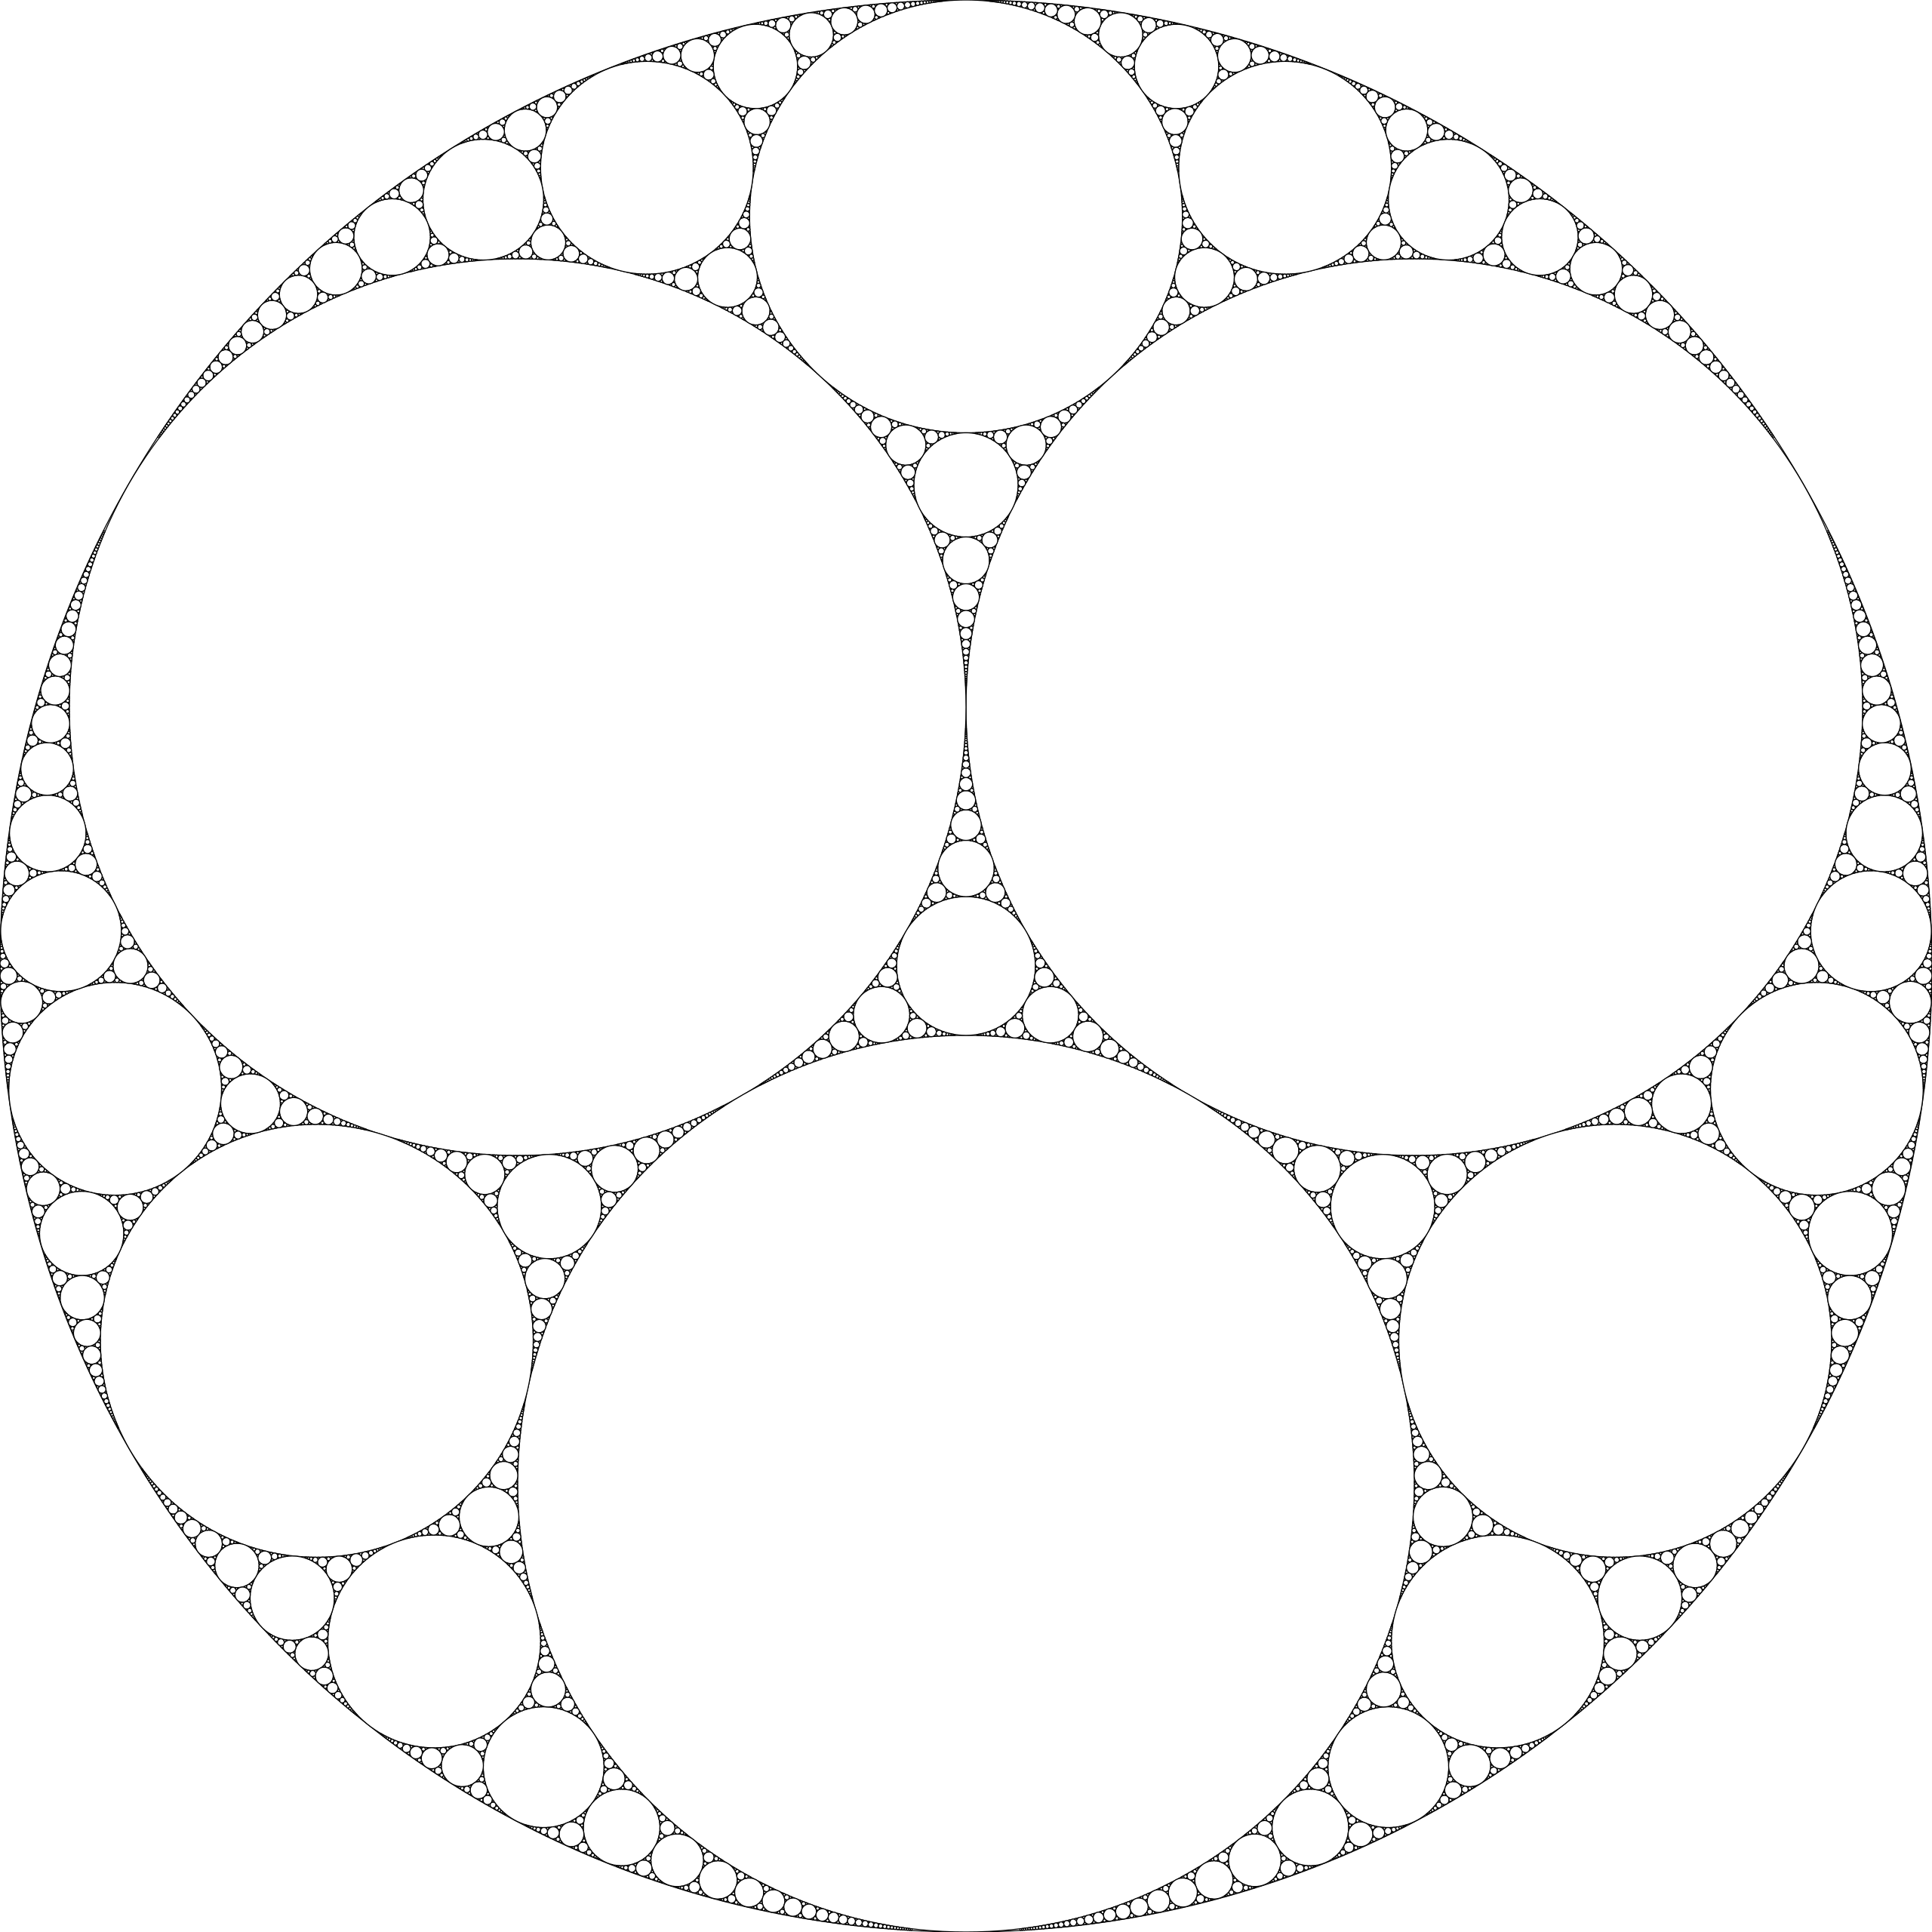
\includegraphics{images/gasket}}
\end{figure}
\end{frame}

\begin{frame}
\frametitle{Knowledge geometry}
A minimal surface of knowledge, every concept is a point, every relation is a line.
\begin{figure}[ht]
\centering
\resizebox{0.5\textwidth}{!}{
\begin{tikzpicture}
\draw (6, 2) node[inner sep=0] {
\includegraphics[width=4in]{images/ennepers.png}};
\node [anchor=225, black] at (9,6) {Geometry};
\node [anchor=225, black] at (9,-3) {Analysis};
\node [anchor=225, black] at (2,6) {Computer Science};
\node [anchor=225, black] at (0,0) {Machine Learning};
\end{tikzpicture}
}
\end{figure}
\end{frame}

\begin{frame}
Thank you!
\end{frame}


\end{document}
